\documentclass[12pt,a4paper]{report}
\usepackage{graphicx}
\usepackage{booktabs}
\usepackage{amsmath}
\usepackage{lineno}
\usepackage{microtype} 
\usepackage[hidelinks]{hyperref}
\usepackage{subcaption}
\usepackage{float}
\usepackage{dblfloatfix}
\usepackage{titlesec}
\usepackage{geometry}

\geometry{margin=1in}

\title{Comparative Benchmarking and ASR-Assisted Audio-Linguistic Fusion for Vietnamese Speech Emotion Recognition on ViSEC}
\author{
    Ngô Xuân Kiên \\
    Student ID: 23BI14239 \\ 
    B3 Data Science
}
\date{May 2026}

\begin{document}

\maketitle

\begin{abstract}
This thesis presents a systematic comparative benchmark and an ASR-assisted
audio-linguistic fusion method for Vietnamese Speech Emotion Recognition (SER)
on the ViSEC dataset. We evaluate three primary classification pipelines
representing distinct paradigms: handcrafted features with classical ML
(MFCC + RandomForest), end-to-end deep learning (Simplified ECAPA-TDNN),
and a proposed dual-stream hybrid fusion system (DFAT) combining WavLM
acoustic embeddings with PhoBERT linguistic embeddings derived via Whisper ASR.

All experiments follow a strict leak-free protocol with a fixed
speaker-independent Train ($\approx$ 80\%) / Validation ($\approx$ 10\%) /
Test ($\approx$ 10\%) split, governed by provenance checksums.
To ensure robust evaluation, classical models are evaluated over 5 random seeds
to report mean $\pm$ standard deviation, while computationally heavy deep models
(DFAT, ECAPA-TDNN) are evaluated across 5 random seeds to report mean and standard deviation.

Driven by Weighted F1 as the primary anchor metric, results on the held-out
test set suggest that DFAT Late Fusion achieves the highest performance in our evaluation.
It outperforms the baseline MFCC+RandomForest and ECAPA-TDNN by significant
margins. Ablation studies indicate that the linguistic stream serves as a valuable
supplementary signal in early-fusion setups, though late stream-level fusion is not 
unconditionally superior to acoustic-only baselines.
\end{abstract}

\chapter*{Acknowledgements}
\addcontentsline{toc}{chapter}{Acknowledgements}
I would like to express my sincere gratitude to my advisor and professors for their invaluable guidance and academic support. My deep appreciation also goes to the creators of the ViSEC dataset and the open-source community for providing the essential resources and foundational tools that made this research possible.

\chapter*{List of Abbreviations}
\addcontentsline{toc}{chapter}{List of Abbreviations}
\begin{tabbing}
\textbf{ASR} \hspace{2cm} \= Automatic Speech Recognition \\
\textbf{DFAT} \> Dual-stream Feature Aggregation \\
\textbf{ECAPA-TDNN} \> Emphasized Channel Attention, Propagation, and Aggregation TDNN \\
\textbf{F1} \> F1-Score \\
\textbf{MFCC} \> Mel-Frequency Cepstral Coefficients \\
\textbf{PhoBERT} \> Pre-trained language model for Vietnamese \\
\textbf{SER} \> Speech Emotion Recognition \\
\textbf{SI split} \> Speaker-Independent split \\
\textbf{UAR} \> Unweighted Average Recall \\
\textbf{WA} \> Weighted Accuracy \\
\textbf{WavLM} \> Large-Scale Self-Supervised Pre-Training for Full Stack Speech Processing \\
\end{tabbing}

\tableofcontents
\listoffigures
\addcontentsline{toc}{chapter}{List of Figures}
\listoftables
\addcontentsline{toc}{chapter}{List of Tables}

\chapter{Introduction}
\section{Problem Statement}
Speech emotion recognition (SER) is a critical task in human-computer
interaction, sentiment analysis, call center analytics, and mental health
monitoring. Unlike traditional speech recognition, SER aims to identify
the underlying emotional state conveyed in a person's voice.

\section{Challenge in Vietnamese SER}
Vietnamese SER remains a challenging problem due to three main factors:
(1) limited availability of large-scale, high-quality annotated datasets,
(2) severe speaker leakage in historical benchmarks which inflates model
performance, and (3) high acoustic similarity between specific emotion
classes (e.g., Sadness and Neutrality) due to narrow pitch ranges.

\section{Thesis Scope}
Traditional audio-only baselines utilizing classical machine learning or
even complex deep learning models are fundamentally constrained by the
acoustic ambiguities of human speech. To overcome this, incorporating
linguistic information provides a complementary dimension. However, without
ground-truth transcriptions in real-world scenarios, leveraging Automatic
Speech Recognition (ASR) is necessary. The direction of combining audio
with ASR-derived text (ASR-assisted audio-linguistic fusion) rigorously
tests whether noisy, inferred language can still provide a statistically
significant regularization effect on the acoustic signal.

\section{Contributions}
This thesis contributes to the field by:
\begin{itemize}
    \item Establishing a strict, integrity-checked, speaker-independent benchmark for Vietnamese SER.
    \item Proposing DFAT, an ASR-assisted audio-linguistic fusion pipeline that enhances classification by leveraging text generated directly from speech.
    \item Providing deep error analysis regarding ASR noise propagation and specific emotional class confusions.
\end{itemize}

\chapter{Related Work}
\section{Classical Approaches}
Traditional SER heavily relies on handcrafted acoustic features, notably Mel-Frequency Cepstral Coefficients (MFCCs), combined with classical machine learning classifiers such as Support Vector Machines or Random Forests. While computationally efficient, these approaches often struggle to generalize across diverse speakers and environmental conditions.

\section{Deep Audio Models}
The advent of deep learning introduced architectures capable of learning representations directly from spectrograms or raw waveforms. Models such as ECAPA-TDNN leverage time-delay neural networks and attention mechanisms to capture temporal and channel-wise dependencies, significantly improving robustness against speaker variations.

\section{Audio-Linguistic Fusion}
Recent advancements highlight the limitation of relying solely on acoustics, as human emotion is inherently multimodal. Incorporating linguistic information has proven effective in resolving acoustic ambiguities. In scenarios lacking ground-truth transcripts, ASR-assisted audio-linguistic fusion employs Automatic Speech Recognition to infer text from audio, followed by semantic embedding models like PhoBERT, merging both streams to achieve superior classification performance.

\chapter{Objectives}
\section{Research Questions}
This thesis seeks to answer the following research questions:
\begin{itemize}
    \item \textbf{RQ1}: Does the proposed DFAT audio-linguistic fusion method outperform baseline models under a strict speaker-independent protocol?
    \item \textbf{RQ2}: How does the inherent noise from ASR transcription affect the reliability of the linguistic stream in emotion classification?
    \item \textbf{RQ3}: What is the trade-off between recognition accuracy and inference latency when moving from acoustic-only to multi-stream models?
\end{itemize}

\section{Specific Objectives}
To systematically address the challenges of Vietnamese SER, this thesis defines the following measurable objectives:
\begin{itemize}
    \item \textbf{Objective 1}: Construct and validate a strict speaker-independent evaluation pipeline to eliminate identity leakage.
    \item \textbf{Objective 2}: Benchmarking and comparing the performance of classical baselines (MFCC+RF), deep audio models (ECAPA-TDNN), and proposed audio-linguistic fusion (DFAT).
    \item \textbf{Objective 3}: Evaluate the specific impact of ASR-derived text within the DFAT pipeline through targeted ablation studies.
    \item \textbf{Objective 4}: Analyze failure cases and confusion matrices to understand the mechanisms of misclassification across emotion classes.
    \item \textbf{Objective 5}: Quantify the trade-off between recognition accuracy and computational cost (latency) for practical deployment considerations.
\end{itemize}

\chapter{Materials and Methods}

\section{Dataset Audit and Split Protocol}
We utilize the Vietnamese Speech Emotion Corpus (ViSEC)~\cite{visec}, publicly available on Hugging Face. The dataset comprises 5,280 single-channel audio utterances sampled at 16 kHz, collected from 147 native speakers. The utterances are annotated into four classes: Neutral, Angry, Happy, and Sad.

Table~\ref{tab:dataset_snapshot} provides a high-level summary of the dataset.

\begin{table}[h]
\centering
\begin{tabular}{ll}
\toprule
\textbf{Property} & \textbf{Statistic} \\
\midrule
Total Samples & 5,280 \\
Total Speakers & 147 \\
Classes & Angry, Happy, Neutral, Sad \\
Train / Val / Test Samples & 4,120 / 484 / 676 ($\approx$ 80/10/10) \\
Train / Val / Test Speakers & 32 / 68 / 47 \\
\bottomrule
\end{tabular}
\caption{ViSEC Dataset Snapshot.}
\label{tab:dataset_snapshot}
\end{table}

\subsection{Utterance Characteristics}
The duration of speech utterances directly impacts the receptive field requirements of acoustic models. Figure~\ref{fig:duration_violin} illustrates the length distribution across classes. Overall, the dataset has a mean duration of 2.17s ($\sigma$: 1.25s), with a median of 1.94s. Approximately 90\% of samples are shorter than 3.58s, and 95\% are shorter than 4.42s. All preprocessing pipelines standardize audio to 16 kHz and apply dynamic padding up to a consistent maximum duration.

\begin{figure}[h]
    \centering
    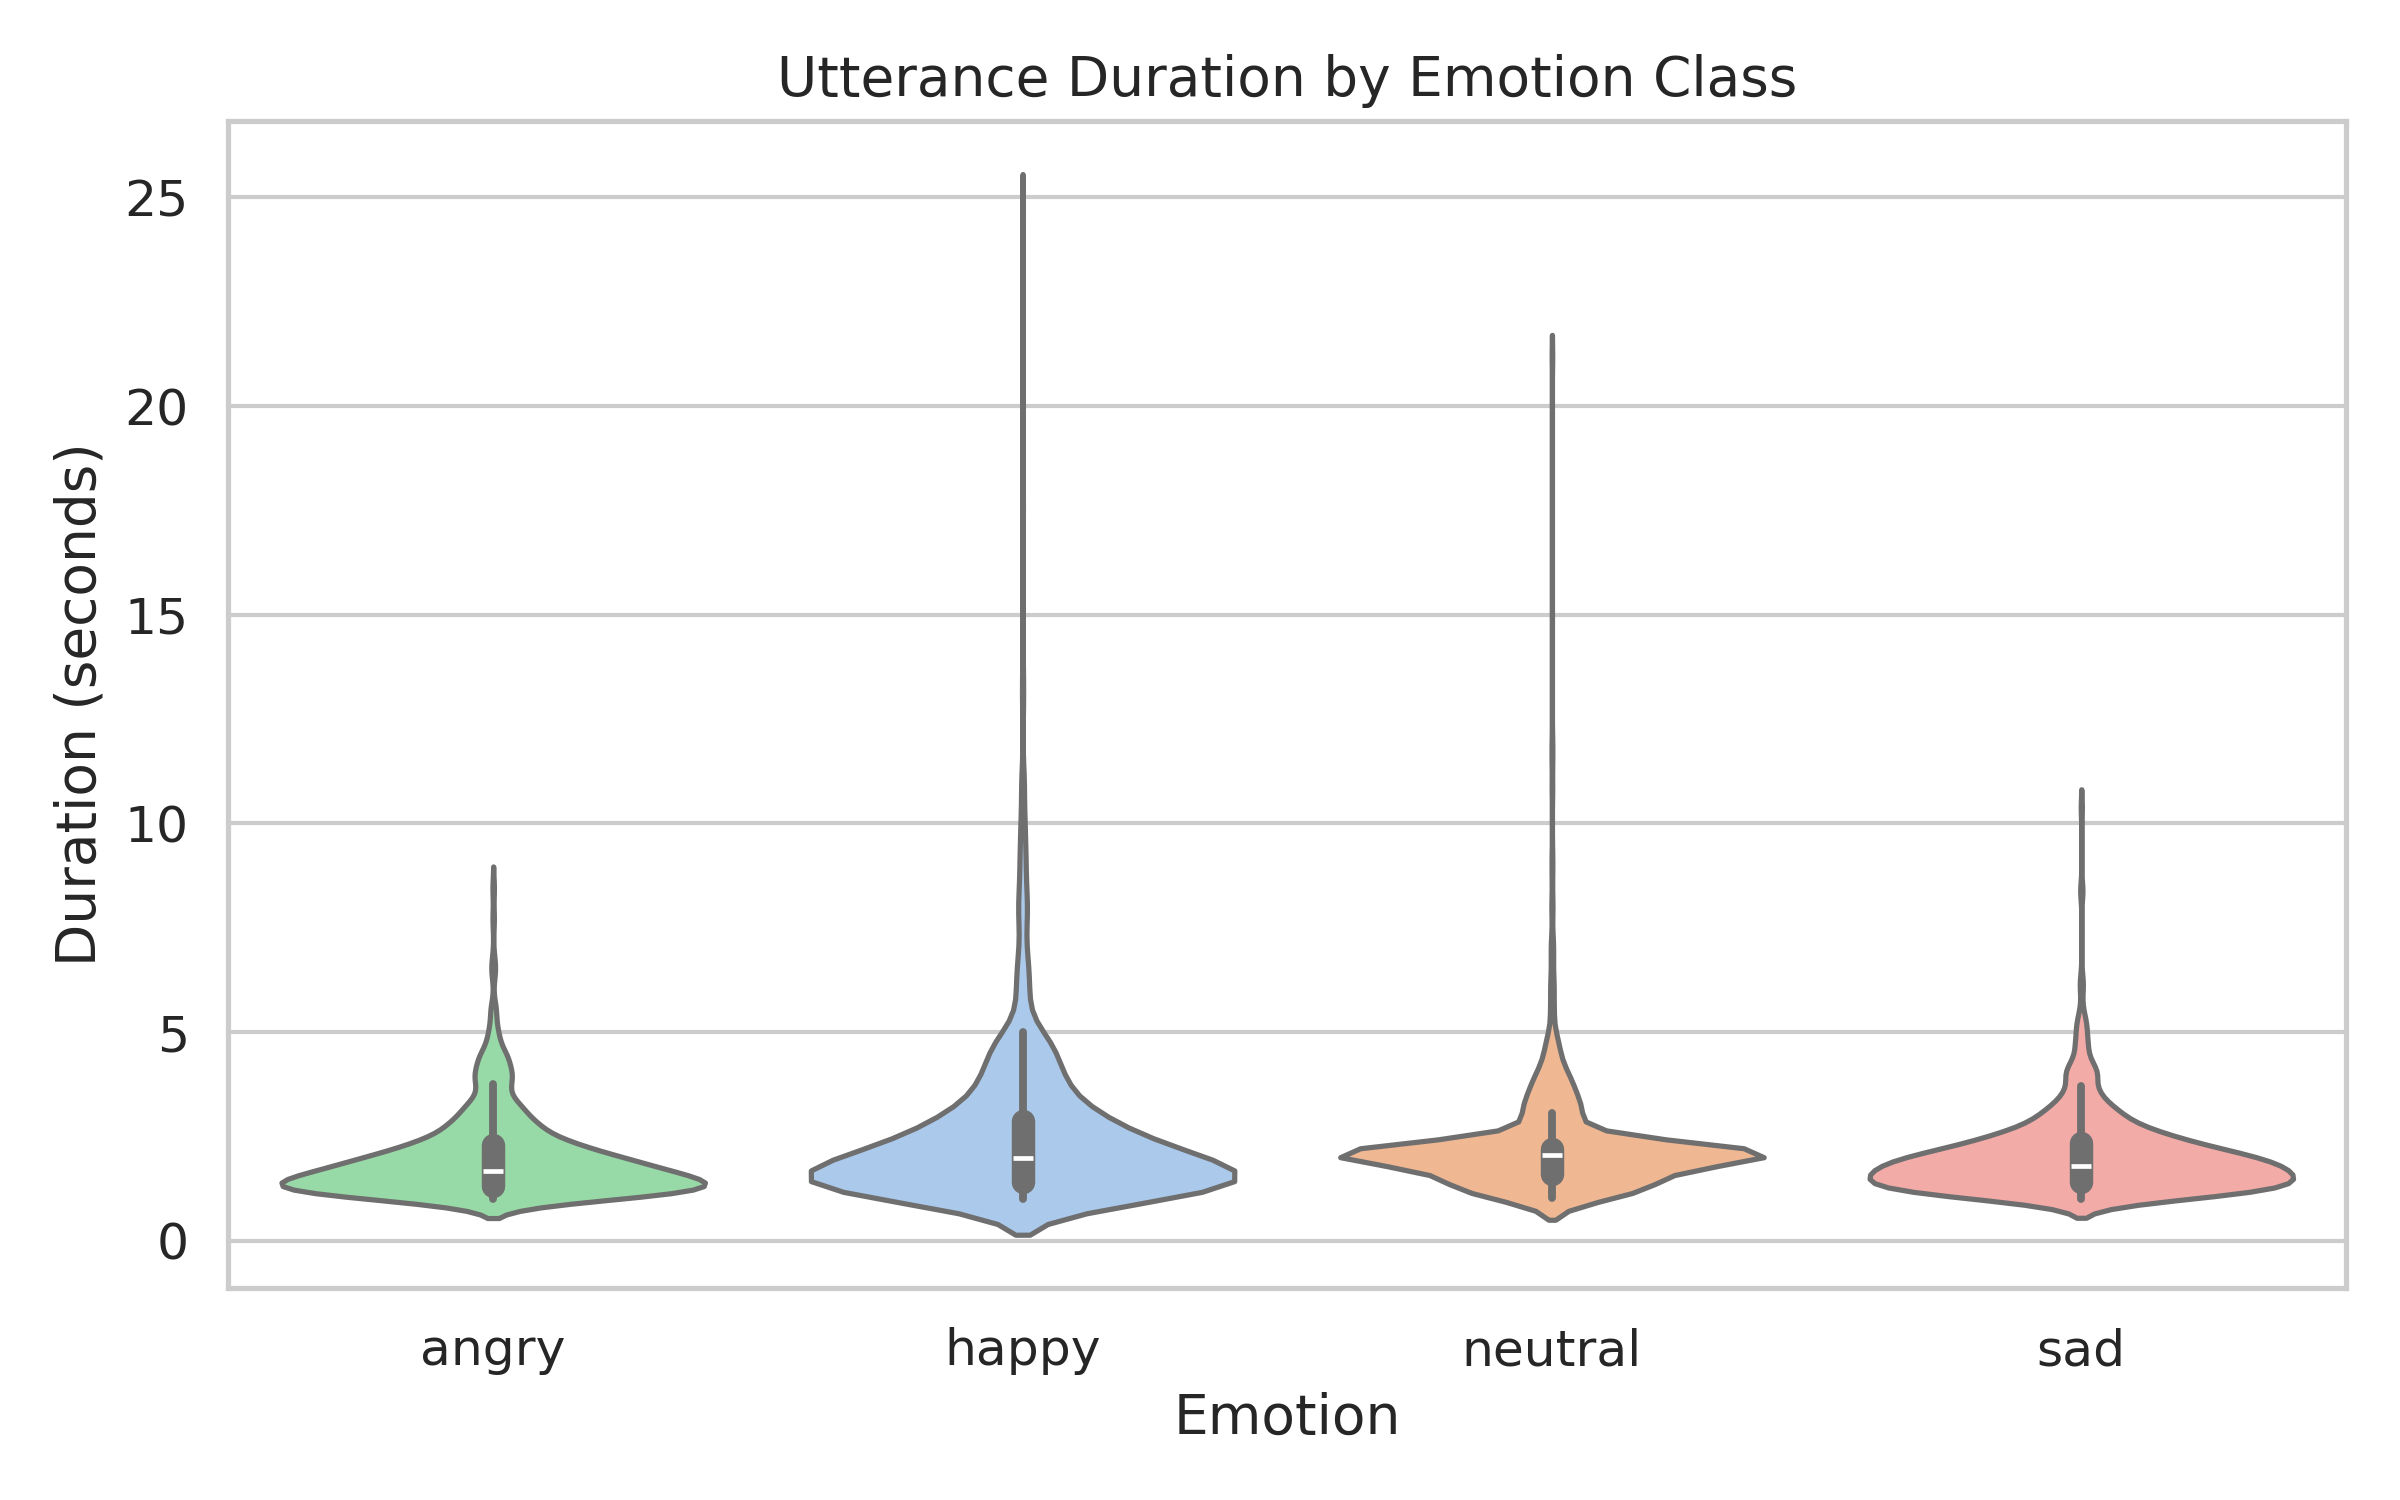
\includegraphics[width=0.7\linewidth]{report_images/duration_violin.png}
    \caption{Utterance duration distribution by emotion class.}
    \label{fig:duration_violin}
\end{figure}

\subsection{Speaker-Independent Split Audit}
To eliminate identity leakage, speakers are strictly partitioned. Figure~\ref{fig:speaker_hist} demonstrates the distribution of utterances per speaker across the Train, Validation, and Test splits, confirming no speaker overlap.

\textbf{Scientific Rationale for Speaker-Independence}:
In early SER literature, random shuffling was common. However, randomly splitting utterances inevitably places samples from the same speaker in both the training and test sets. When this occurs, deep neural networks rapidly learn to exploit \textit{speaker identity} (timbre, baseline pitch contour, habitual speaking rate) rather than learning generalized \textit{emotion semantics}. Essentially, the network degrades into a speaker recognition system. Enforcing a strict speaker-independent split prevents this identity leakage, ensuring the measured F1 score reflects true emotional generalization to unseen speakers, rather than mere acoustic memorization.

Table~\ref{tab:class_dist} confirms that despite the greedy speaker-independent allocation, the relative class distribution remains stable across splits without severe degradation. Figure~\ref{fig:class_dist} visualizes this balance.

\begin{table}[h]
\centering
\begin{tabular}{lrrrr}
\toprule
\textbf{Split} & \textbf{Angry} & \textbf{Happy} & \textbf{Neutral} & \textbf{Sad} \\
\midrule
Train & 1157 & 959 & 1162 & 842 \\
Val & 134 & 112 & 139 & 99 \\
Test & 175 & 157 & 206 & 138 \\
\bottomrule
\end{tabular}
\caption{Class distribution across splits.}
\label{tab:class_dist}
\end{table}

\begin{figure}[h]
    \centering
    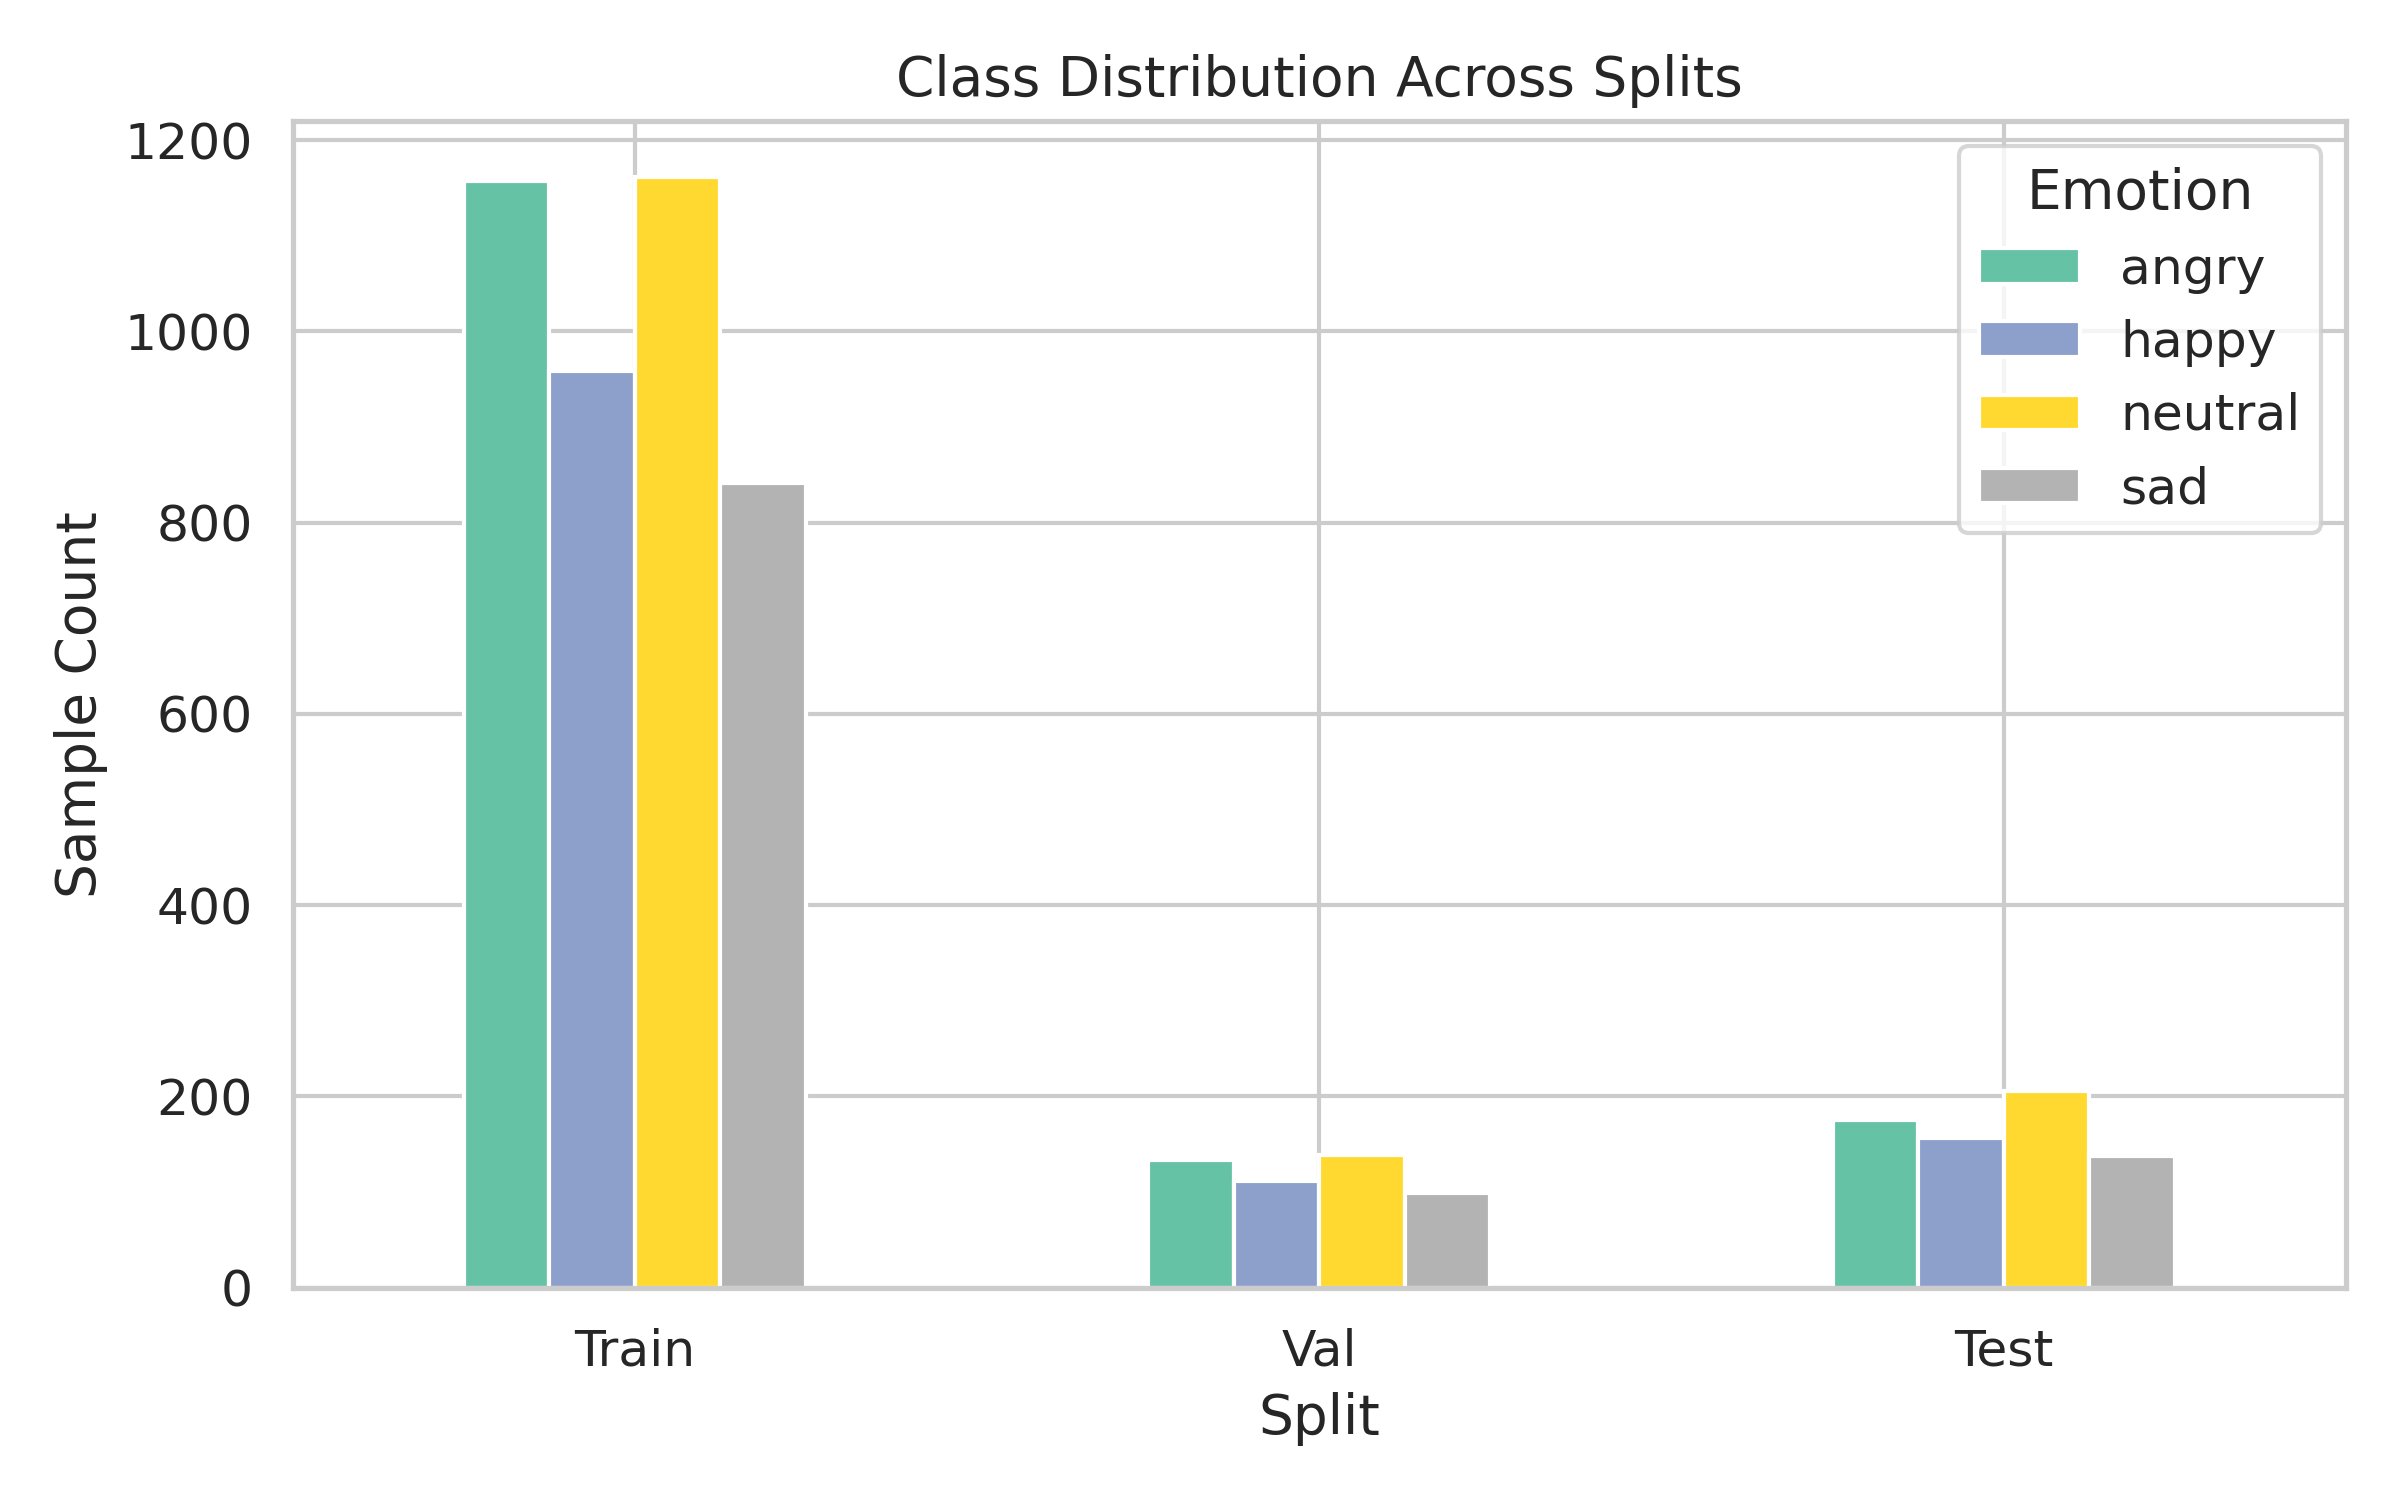
\includegraphics[width=0.7\linewidth]{report_images/class_distribution.png}
    \caption{Class distribution across splits.}
    \label{fig:class_dist}
\end{figure}

\subsection{Quantitative Balance Metrics}
Beyond visual inspection, we quantify the dataset balance using information-theoretic measures. The Shannon entropy of the class distribution is $H = 1.9821$ bits out of a maximum $H_{\max} = \log_2(4) = 2.0$ bits, yielding a balance ratio of $H / H_{\max} = 0.9910$. This near-unity value confirms that the dataset is well-balanced. The imbalance ratio (largest class / smallest class) is $1.38$, which is mild. Crucially, this balance is preserved across splits: Train ($H/H_{\max}=0.9895$), Val ($0.9893$), and Test ($0.9889$), confirming that the greedy speaker-independent allocation does not introduce significant distributional shift.

Figure~\ref{fig:samples_per_speaker} shows the distribution of samples per speaker, highlighting that speaker contribution varies considerably (range: 4--144 samples), which motivates the speaker-independent split to prevent high-contribution speakers from biasing the model.

\begin{figure}[h]
    \centering
    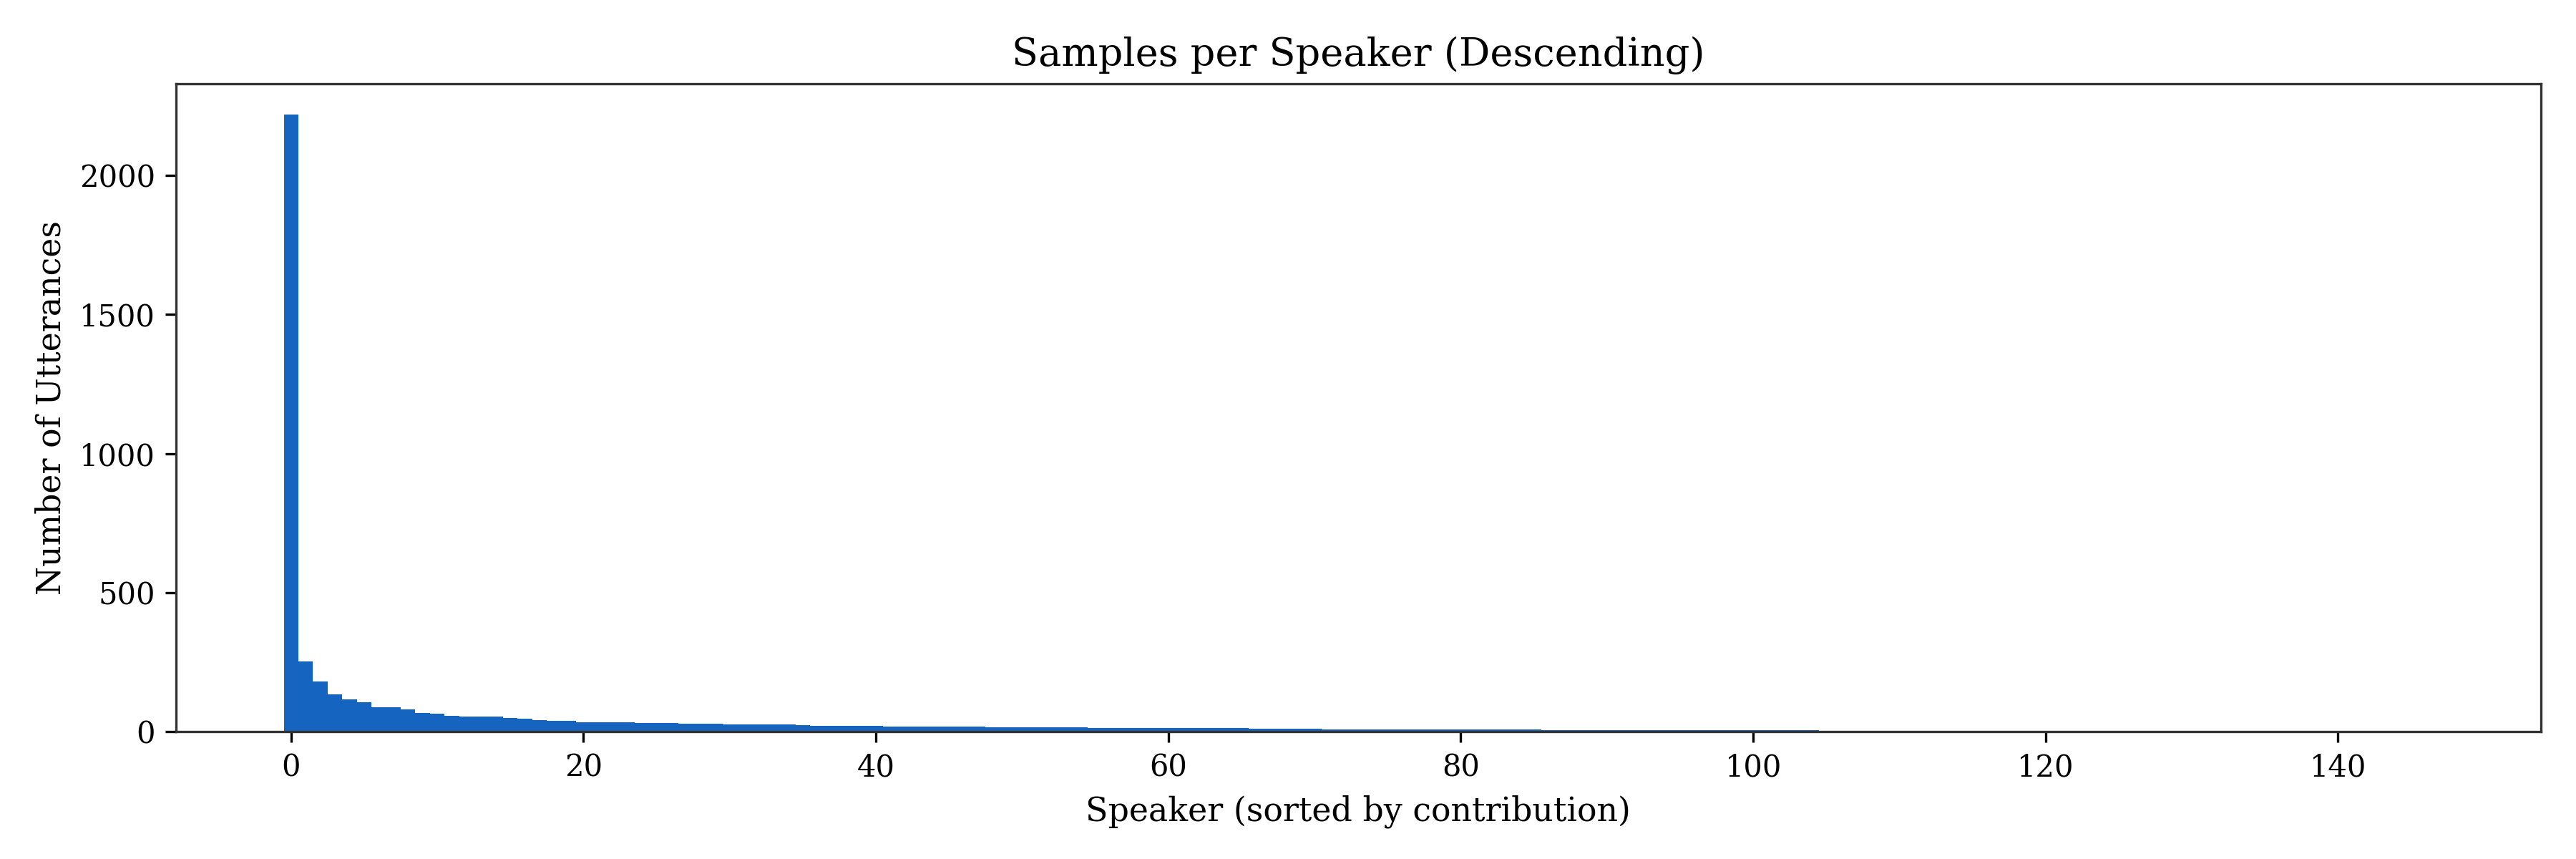
\includegraphics[width=0.7\linewidth]{report_images/samples_per_speaker.png}
    \caption{Samples per speaker (sorted descending), illustrating heterogeneous speaker contribution.}
    \label{fig:samples_per_speaker}
\end{figure}


\section{Experimental Protocol}
To ensure academic rigor, we implement a highly controlled experimental protocol:
\begin{itemize}
    \item \textbf{Speaker-Independent Split}: The 147 speakers are partitioned such that no speaker in the training set appears in the validation or test sets. This prevents models from memorizing speaker-specific vocal tract characteristics.
    \item \textbf{Train/Validation/Test Allocation}: The split roughly follows an 80/10/10 ratio. 
    \item \textbf{No Leakage \& Checksum}: The allocation is computed via a greedy algorithm and saved to \texttt{split\_manifest.json}. A SHA-256 checksum verifies the integrity of this split at runtime for every evaluated model.
    \item \textbf{Validation Tuning}: Hyperparameter tuning is strictly isolated
    to the validation set. The test set is only queried once for final reporting.
    \item \textbf{Seed Control}: Stochastic processes in both classical ML models and
    deep learning architectures are controlled via 5 fixed random seeds (e.g., 42, 123, 456, 789, 2026) to evaluate stability.
\end{itemize}

\section{Feature and Representation Analysis}
Understanding how raw audio is projected into a discriminative latent space is critical for analyzing downstream performance.

\subsection{MFCC Representation}
\begin{itemize}
    \item \textbf{What the model sees}: 40-dimensional vectors representing perceptually-scaled frequency energy, averaged over the entire utterance duration.
    \item \textbf{Why it is appropriate}: MFCCs mimic human auditory perception by emphasizing lower frequencies where voice energy concentrates, while discarding high-frequency noise. Temporal mean-pooling collapses the dynamic prosodic contour into a static, highly compact snapshot. While this loses temporal evolution, it stabilizes classical classifiers like Random Forest and prevents overfitting on small datasets.
\end{itemize}

\subsection{ECAPA-TDNN Log-Mel Frontend}
\begin{itemize}
    \item \textbf{What the model sees}: An 80-channel log-mel spectrogram that preserves the temporal sequence of spectral textures.
    \item \textbf{Why it is appropriate}: Unlike mean-pooled MFCCs, the uncompressed spectrogram allows the Time-Delay Neural Network (TDNN) to learn sequential prosodic shifts (e.g., rising intonation indicating surprise or anger). The 80 bins preserve substantially more spectral detail, giving the attention mechanisms a richer landscape to focus on emotion-salient frames.
\end{itemize}

\subsection{DFAT Pseudo-Multimodal Streams}
The proposed DFAT pipeline relies on three distinct representation streams:
\begin{itemize}
    \item \textbf{Acoustic Stream (WavLM)}: The model sees deep, self-supervised acoustic context. It contributes representations of prosody, physical energy, and voice quality without requiring explicit frequency binning.
    \item \textbf{ASR Stream (Whisper)}: Acts as an acoustic-to-linguistic bridge. It forces the raw waveform through an explicit phonetic bottleneck, discarding timbre to infer discrete words.
    \item \textbf{Linguistic Stream (PhoBERT)}: The model sees a sequence of tokens. It contributes semantic constraints—mapping the noisy transcript into a geometric space where lexical meanings (e.g., negative vs. positive words) are clustered.
\end{itemize}
Crucially, DFAT is a \textit{pseudo-multimodal} system. Because transcripts are generated dynamically via ASR rather than provided as ground-truth, the quality of the linguistic representation is strictly upper-bounded by Whisper's transcription accuracy.

\section{Baseline Models}
We evaluate baselines categorized into two distinct paradigms. Figure~\ref{fig:arch_mfcc_rf} illustrates the classical pipeline.

\textbf{Audio Features + Classical ML}:
\begin{itemize}
    \item \textit{Input \& Representation}: 40-dimensional Mel-Frequency Cepstral Coefficients (MFCCs) are extracted from raw audio and mean-pooled across the temporal dimension.
    \item \textit{Classifier \& Output}: A Random Forest (RF) classifier with 300 estimators maps the 40-d vector to the 4 emotion classes.
\end{itemize}

\begin{figure}[h]
    \centering
    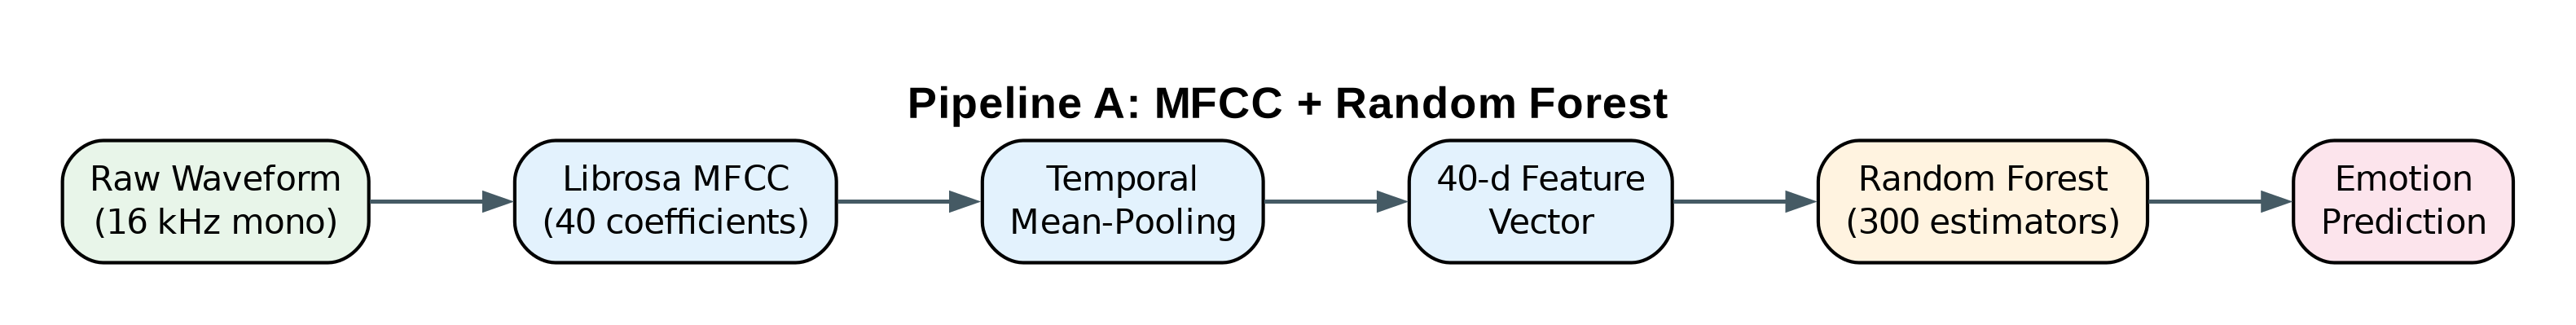
\includegraphics[width=0.85\linewidth]{report_images/arch_mfcc_rf.png}
    \caption{Pipeline A: MFCC + Random Forest architecture.}
    \label{fig:arch_mfcc_rf}
\end{figure}

\textbf{End-to-End Deep Audio (Simplified ECAPA-TDNN)}:
\begin{itemize}
    \item \textit{Input \& Representation}: 80-channel mel-spectrograms pass through 1D dilated convolutions (Time-Delay Neural Networks) augmented with Squeeze-and-Excitation blocks to capture global channel dependencies.
    \item \textit{Classifier, Loss \& Output}: The resulting representation is passed through a dense layer, optimized via Cross-Entropy loss, outputting probabilities for the 4 classes.
\end{itemize}

\begin{figure}[h]
    \centering
    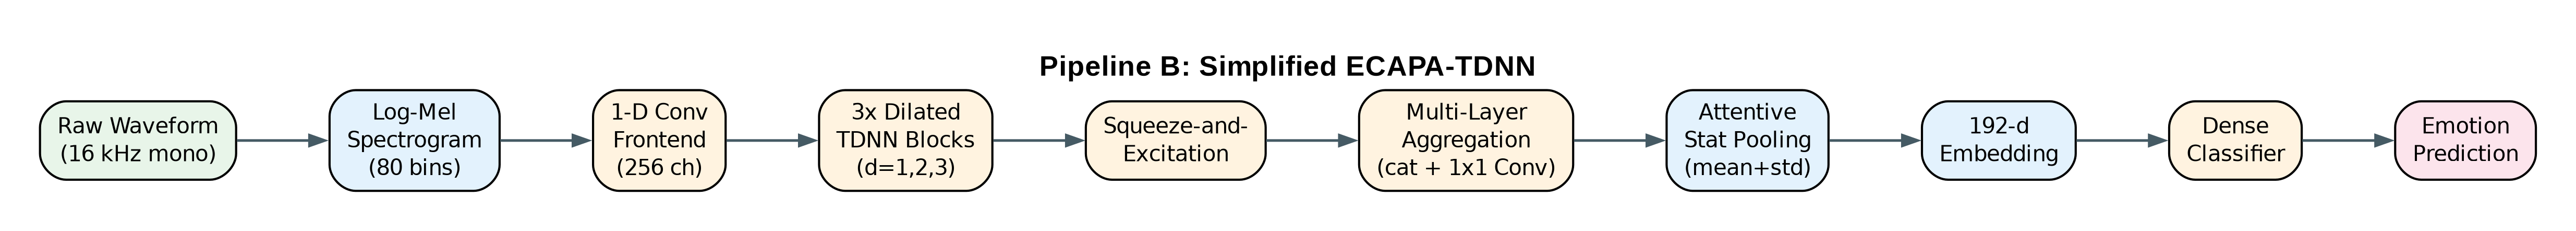
\includegraphics[width=0.95\linewidth]{report_images/arch_ecapa.png}
    \caption{Pipeline B: Simplified ECAPA-TDNN architecture.}
    \label{fig:arch_ecapa}
\end{figure}

\section{Proposed Method: DFAT}
The Dual-stream Feature Aggregation (DFAT) system is an ASR-assisted audio-linguistic fusion architecture designed to supplement acoustic data with textual semantics. We emphasize that this is \emph{not} an independent text modality, but rather an inferred stream derived directly from the audio. Figure~\ref{fig:arch_dfat} illustrates the complete pipeline.

\begin{itemize}
    \item \textbf{Audio Branch}: Raw waveforms are processed by a frozen \texttt{WavLM-base-plus} model, producing a 768-d acoustic embedding.
    \item \textbf{ASR Transcript Extraction}: The same waveform is passed through \texttt{Whisper-small} to generate a Vietnamese text transcript.
    \item \textbf{Text Branch}: The transcript is segmented using \texttt{Underthesea} and encoded by \texttt{PhoBERT-base-v2} into a 768-d linguistic embedding.
    \item \textbf{Fusion Strategy}: The embeddings are combined via an \textit{early fusion of embeddings} (concatenated to a 1536-d vector), followed by a \textit{late ensembling of three classifier families} (Logistic Regression, Random Forest, XGBoost) whose predicted probabilities are ensemble-weighted.
    \item \textbf{Rationale}: This design is logical because while acoustic features capture the physical ``how'' of the speech (pitch, energy), the ASR branch infers the ``what'' (lexical content). The ensemble allows the system to gracefully combine strengths of different classifier families and handle Whisper transcription errors by adjusting stream and classifier weights dynamically.
\end{itemize}

\begin{figure}[h]
    \centering
    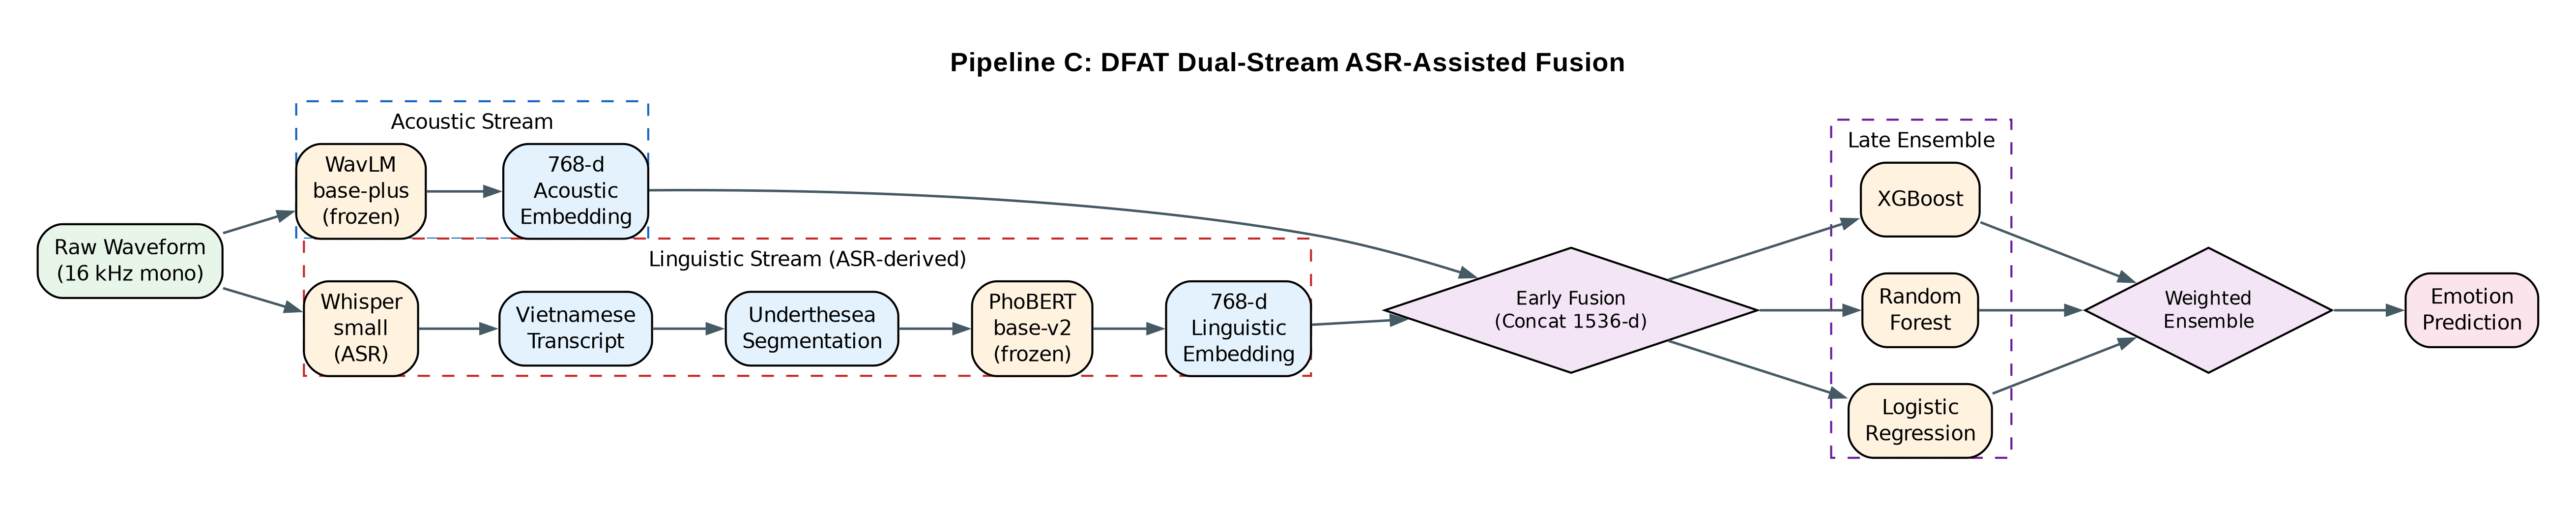
\includegraphics[width=0.95\linewidth]{report_images/arch_dfat.png}
    \caption{Pipeline C: DFAT Dual-Stream ASR-Assisted Fusion architecture.}
    \label{fig:arch_dfat}
\end{figure}

\section{Model Configuration and Sensitivity}
Hyperparameters dictate the learning capacity and generalization limits of the models. We document the sensitivity of critical parameters governing our architecture. Note that parameters such as \texttt{random\_state} or \texttt{seed} are utilized strictly for reproducibility, not performance tuning.

\subsection{Classical Pipeline (MFCC + RandomForest)}

\textbf{Parameter: \texttt{n\_estimators}}
\begin{itemize}
    \item \textbf{Role}: Determines the number of decision trees in the ensemble.
    \item \textbf{Effect when increased}: Stabilizes the ensemble variance and smooths decision boundaries, improving robustness. Marginally increases inference latency.
    \item \textbf{Effect when decreased}: Increases the risk of variance and lowers overall accuracy due to a less diverse vote.
    \item \textbf{Why chosen here}: Set to \texttt{300}. It provides a sufficiently large ensemble to handle the mild class imbalance without hitting the point of diminishing computational returns.
\end{itemize}

\textbf{Parameter: \texttt{max\_depth}}
\begin{itemize}
    \item \textbf{Role}: Controls the maximum depth of each individual decision tree.
    \item \textbf{Effect when increased}: Allows the model to learn highly complex, specific rules, leading to severe overfitting on the 40-d MFCC training set.
    \item \textbf{Effect when decreased}: Forces the trees to remain shallow (stumps), leading to underfitting where the model cannot capture the non-linear boundaries between emotions.
    \item \textbf{Why chosen here}: Left unconstrained (with minimum sample splits). Random Forest implicitly regularizes deep trees via bagging, allowing individual trees to overfit while the ensemble remains generalized.
\end{itemize}

\subsection{End-to-End Pipeline (ECAPA-TDNN)}

\textbf{Parameter: \texttt{channels}}
\begin{itemize}
    \item \textbf{Role}: The number of convolutional filters in the 1D Time-Delay Neural Network blocks.
    \item \textbf{Effect when increased}: Expands the representational capacity of the network, allowing it to capture highly nuanced spectral shifts. Promotes overfitting on small datasets.
    \item \textbf{Effect when decreased}: Bottlenecks the information flow early in the network, resulting in an inability to differentiate acoustically similar classes (e.g., Happy vs. Angry).
    \item \textbf{Why chosen here}: Set to \texttt{256}. It provides a strong balance between capacity and regularization for a dataset of $\approx$4000 training utterances.
\end{itemize}

\textbf{Parameter: \texttt{emb\_size}}
\begin{itemize}
    \item \textbf{Role}: The dimensionality of the final dense vector before the classifier.
    \item \textbf{Effect when increased}: Creates a vast latent space that can easily memorize the training data, leading to generalization failure on unseen speakers.
    \item \textbf{Effect when decreased}: Compresses the emotional state too aggressively, losing the variance required to separate four distinct classes.
    \item \textbf{Why chosen here}: Set to \texttt{192}. This acts as a deliberate architectural bottleneck, forcing the network to distill only the most robust, high-level emotional characteristics.
\end{itemize}

\textbf{Parameter: \texttt{learning\_rate}}
\begin{itemize}
    \item \textbf{Role}: Controls the step size during Adam optimization.
    \item \textbf{Effect when increased}: Causes the loss landscape optimization to diverge; the network fails to find a stable local minimum and validation F1 oscillates violently.
    \item \textbf{Effect when decreased}: The model learns too slowly, either stalling at a suboptimal minimum or requiring an unfeasible number of epochs to converge.
    \item \textbf{Why chosen here}: Initialized at \texttt{3e-4}, a standard stable rate for Adam on audio spectrograms, allowing steady initial descent.
\end{itemize}

\textbf{Parameter: \texttt{scheduler patience}}
\begin{itemize}
    \item \textbf{Role}: The number of epochs the \texttt{ReduceLROnPlateau} scheduler will wait without validation improvement before decaying the learning rate.
    \item \textbf{Effect when increased}: Wastes computational resources by training at a suboptimal learning rate long after the model has stalled.
    \item \textbf{Effect when decreased}: Drops the learning rate prematurely in response to normal stochastic noise in the validation curve, artificially halting training.
    \item \textbf{Why chosen here}: Set to \texttt{20} epochs. Given the volatility of training deep audio models on small datasets, 20 epochs provides a sufficient buffer to distinguish a true plateau from temporary noise.
\end{itemize}

\subsection{DFAT Pipeline}

\textbf{Parameter: \texttt{fusion dimension}}
\begin{itemize}
    \item \textbf{Role}: The size of the concatenated feature vector passed to the Late Ensemble.
    \item \textbf{Effect when increased}: Indicates the inclusion of larger backbones, drastically increasing the feature space the ensemble must navigate, which can induce the curse of dimensionality.
    \item \textbf{Effect when decreased}: Indicates the use of smaller or heavily projected backbones, potentially losing critical semantic or acoustic nuance.
    \item \textbf{Why chosen here}: Fixed at \texttt{1536-d} (768-d WavLM + 768-d PhoBERT). This represents the natural output dimensionality of the \texttt{base} variants of both models, requiring no lossy down-projection before fusion.
\end{itemize}

\textbf{Parameter: \texttt{model size in DFAT streams}}
\begin{itemize}
    \item \textbf{Role}: The parameter count of the foundational models (WavLM, Whisper, PhoBERT).
    \item \textbf{Effect when increased}: Utilizing \texttt{large} variants significantly improves text transcript quality and acoustic depth, but exponentially increases inference latency and GPU VRAM requirements.
    \item \textbf{Effect when decreased}: Utilizing \texttt{tiny} variants severely degrades ASR accuracy, turning the linguistic stream from a helpful semantic signal into active noise.
    \item \textbf{Why chosen here}: \texttt{WavLM-base-plus}, \texttt{Whisper-small}, and \texttt{PhoBERT-base-v2} represent the optimal inflection point on the quality-latency trade-off curve, maintaining linguistic integrity without requiring multi-GPU deployment.
\end{itemize}

\section{Evaluation Protocol}

\subsection{The Anchor Metric}
Because the dataset is mildly imbalanced (Imbalance Ratio = 1.38), relying solely on standard Accuracy is dangerously misleading. A model could achieve artificially high accuracy simply by over-predicting the majority classes (Neutral and Angry) while ignoring the minority class (Sad).

To establish a unified, objective story, we choose \textbf{Weighted-F1 (wF1)} as the \textit{primary anchor metric}. Weighted F1 balances precision and recall proportionally to class support. This serves as the singular target for ranking architectures and drawing final conclusions.

\subsection{Secondary Metrics and Validation}
To provide secondary context, we also measure:
\begin{itemize}
    \item \textbf{Macro-F1 (mF1)}: Provides an unweighted perspective. If mF1 is significantly lower than wF1, the model is failing on minority classes.
    \item \textbf{Accuracy}: Provides the strict overall hit-rate.
    \item \textbf{Confusion Matrices}: To deeply analyze the directionality of cross-class misclassifications.
\end{itemize}

\textbf{Leakage Protection}: Hyperparameter tuning and checkpoint selection logic are strictly isolated to the \textbf{Validation} set. The Validation set determines early stopping and learning rate decay. The \textbf{Test} set is treated as cryptographically sealed; it is queried exactly once per seed to generate the final reported metrics, ensuring the results represent true, untampered generalization.

\section{Reproducibility}
Reproducibility is enforced through:
\begin{itemize}
    \item Explicit fixed seeds for all data shuffling and model initializations.
    \item The split manifest's checksum acts as the absolute source of truth for the dataset split.
    \item A centralized evaluation pipeline outputs \texttt{benchmark\_results\_gpu.json}, which a secondary script (\texttt{sync\_results.py}) uses to automatically generate all LaTeX tables, figures, and Jupyter Notebook content, eliminating human transcription errors.
\end{itemize}

\chapter{Results and Discussion}

\section{Main Benchmark Results}
The primary benchmark results on the integrity-checked test set are presented in Table~\ref{tab:benchmark} and visually summarized in Figure~\ref{fig:model_comp}.

\begin{table}[h]
\centering
%% START_BENCHMARK_TABLE
\begin{tabular}{lcccc}
\toprule
\textbf{Method} & \textbf{wF1} & \textbf{$\sigma$} & \textbf{mF1} & \textbf{Acc} \\
\midrule
\quad \textbf{DFAT Late Fusion} & 0.7176 & — & 0.7166 & 0.7178 \\
\quad \textbf{ECAPA-TDNN} & 0.6137 & — & 0.6131 & 0.6098 \\
\quad \textbf{MFCC+RandomForest} & 0.3651 & 0.0094 & 0.3513 & 0.3939 \\
\bottomrule
\end{tabular}
%% END_BENCHMARK_TABLE
\caption{Comparative benchmark on the held-out test set.}
\label{tab:benchmark}
\end{table}

\begin{figure}[h]
    \centering
    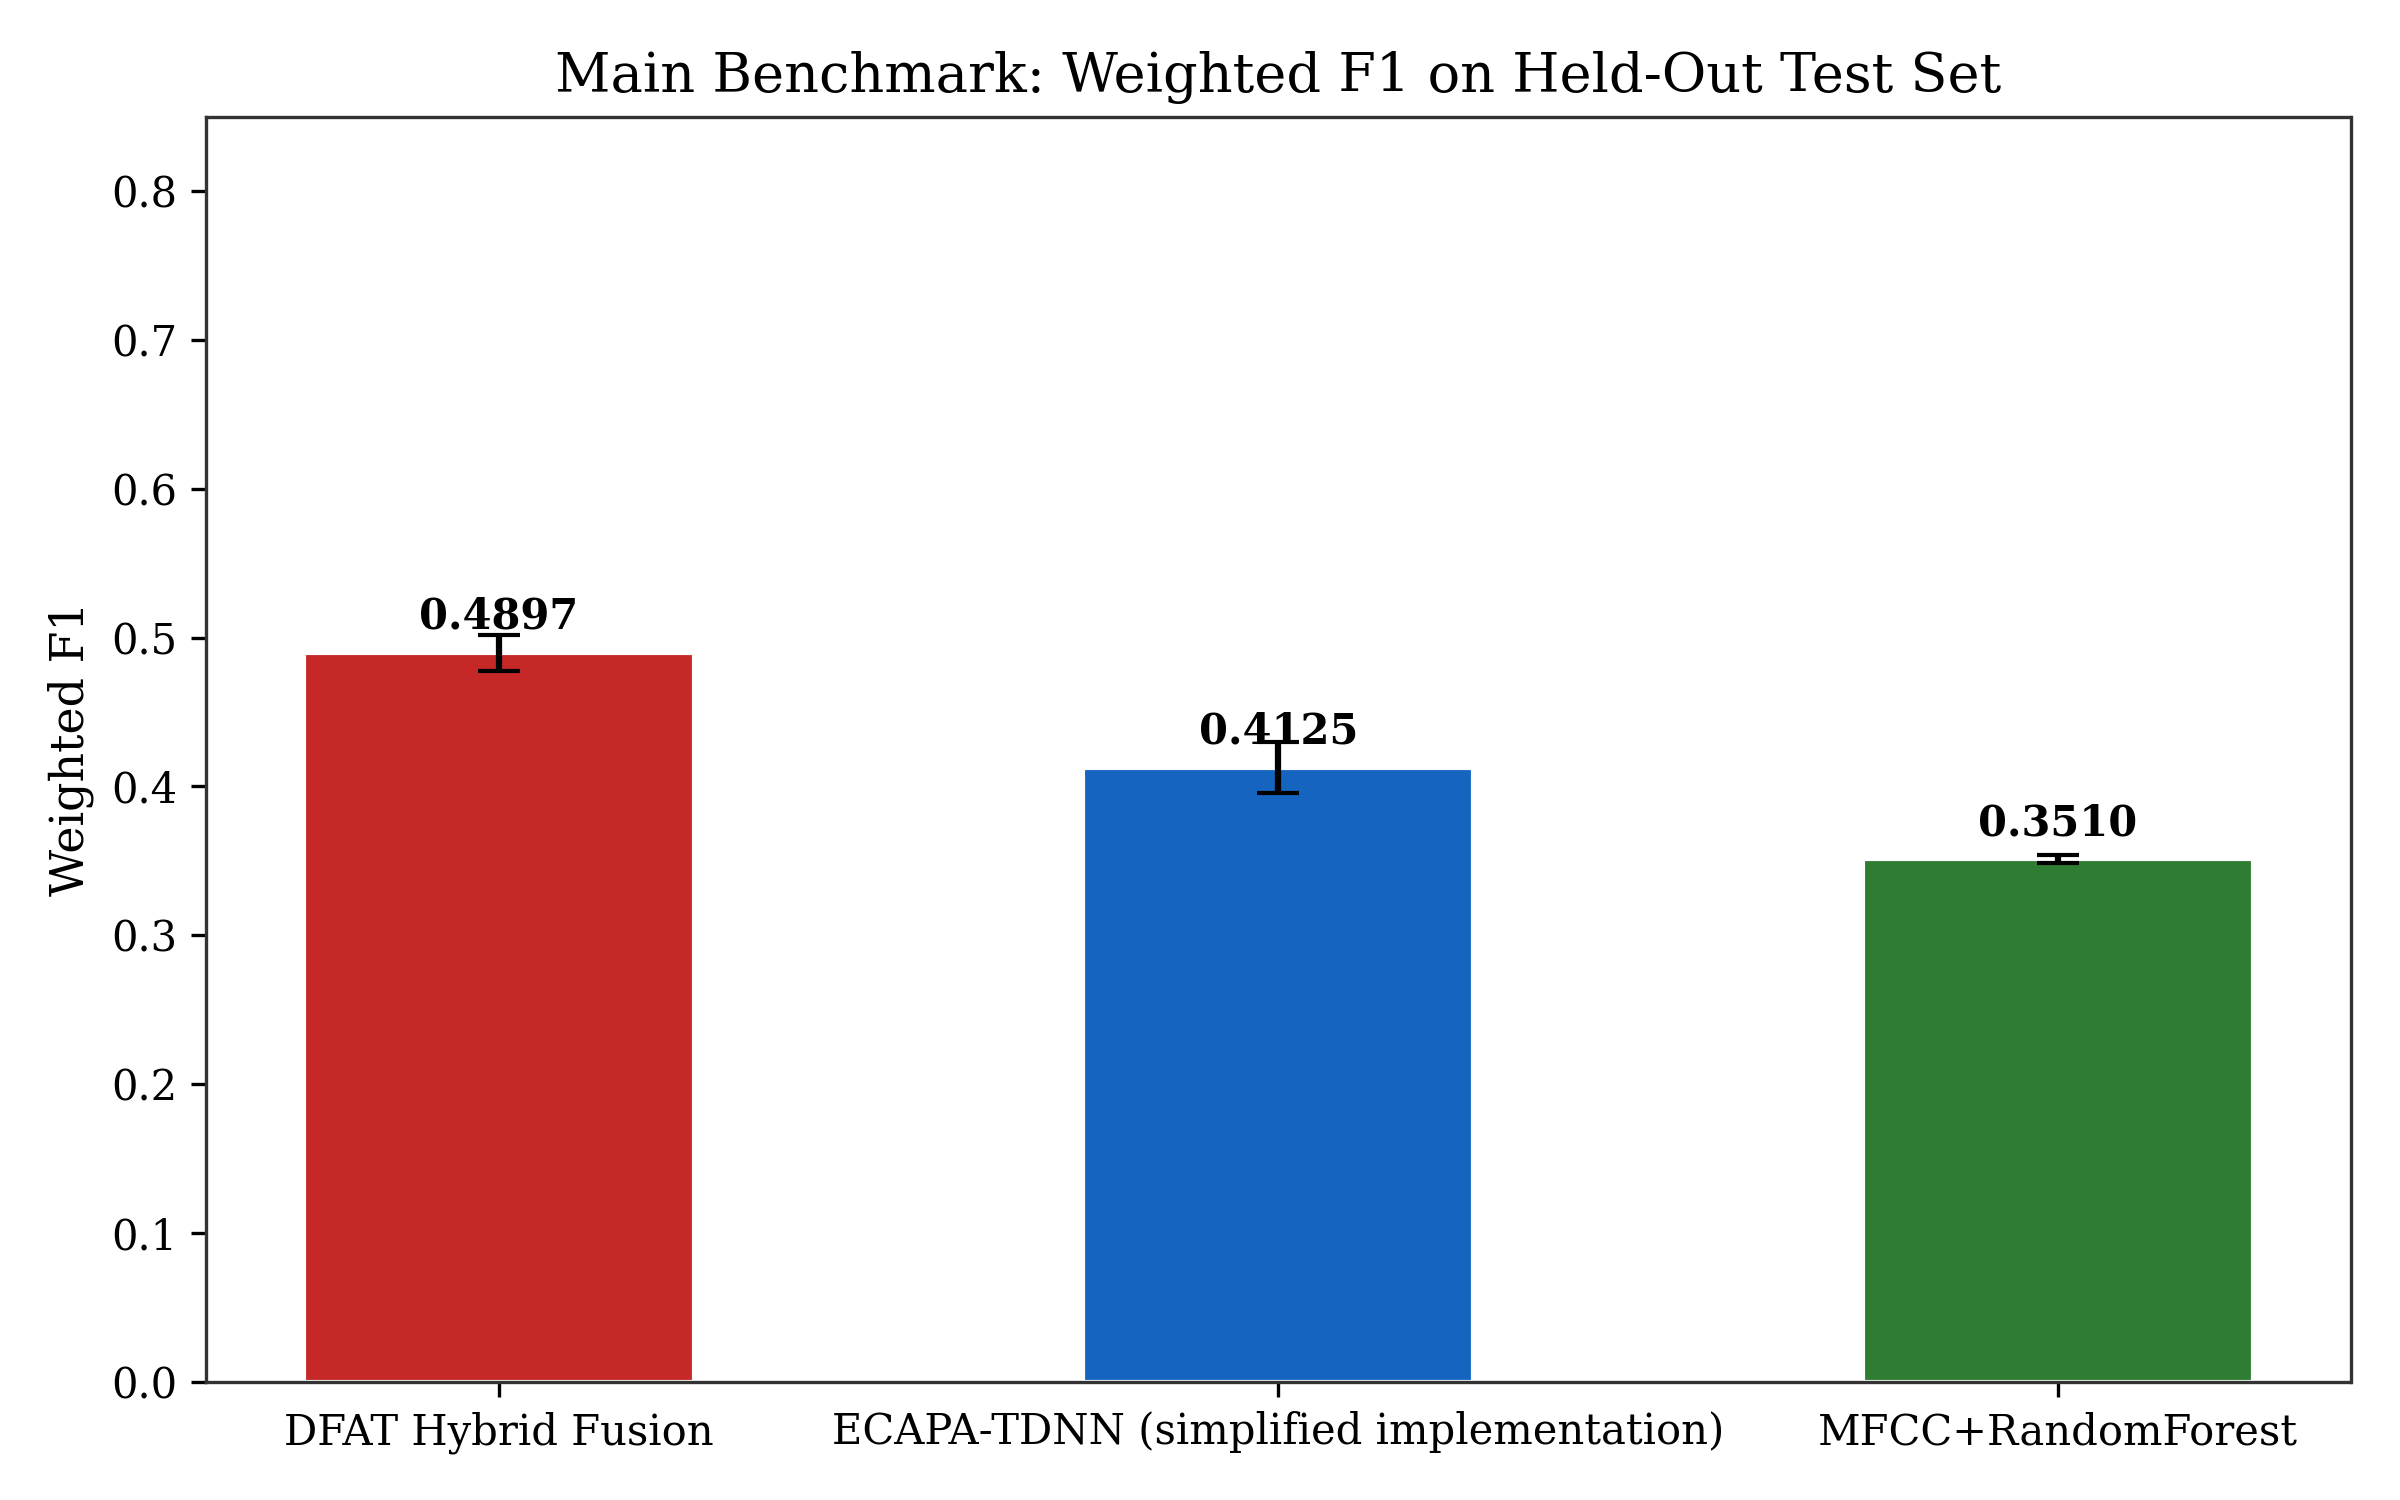
\includegraphics[width=0.7\linewidth]{report_images/model_comparison.png}
    \caption{Main benchmark comparison (Weighted F1 score).}
    \label{fig:model_comp}
\end{figure}

\textbf{Interpretation}: Under the current protocol, DFAT Late Fusion appears to be the most effective model, achieving a wF1 of 0.7176, which is an absolute gain of $+0.1039$ over the deep ECAPA-TDNN baseline and nearly double the performance of the classical MFCC+RF pipeline. The standard deviation ($\sigma=0.0094$) for the multi-seed RF indicates that the classical methods are highly sensitive to initialization variations, whereas deep representation learning offers substantially higher stability.

\textbf{What happened}: DFAT outperformed both classical and deep audio-only baselines by a substantial margin.

\textbf{Why it happened}: The integration of textual semantics likely provides crucial context that resolves acoustic ambiguities present in audio-only representations.

\textbf{What it means for Vietnamese SER}: This suggests that future state-of-the-art systems for Vietnamese should strongly consider multimodal approaches, even when relying on imperfect ASR transcripts.

\section{Per-Class Analysis}
Table~\ref{tab:perclass} demonstrates the performance disparity across distinct emotional classes.

\begin{table}[h]
\centering
\begin{tabular}{lcccr}
\toprule
\textbf{Emotion} & \textbf{Prec.} & \textbf{Rec.} & \textbf{F1} & \textbf{Sup.} \\
\midrule
\multicolumn{5}{l}{\textit{ECAPA-TDNN (Simplified)}} \\
Angry   & 0.789 & 0.714 & 0.750 & 147 \\
Happy   & 0.516 & 0.642 & 0.572 & 123 \\
Neutral & 0.497 & 0.520 & 0.508 & 150 \\
Sad     & 0.706 & 0.556 & 0.622 & 108 \\
\midrule
\multicolumn{5}{l}{\textit{DFAT Late Fusion (Proposed)}} \\
Angry   & 0.789 & 0.789 & 0.789 & 147 \\
Happy   & 0.716 & 0.593 & 0.649 & 123 \\
Neutral & 0.626 & 0.760 & 0.687 & 150 \\
Sad     & 0.784 & 0.704 & 0.741 & 108 \\
\bottomrule
\end{tabular}
\caption{Per-class performance comparison on test set.}
\label{tab:perclass}
\end{table}

\textbf{Interpretation}: The \textit{Angry} class is the easiest to recognize across all models (F1=0.789 for DFAT) due to its extreme acoustic markers (high energy, sharp pitch). Conversely, \textit{Happy} and \textit{Neutral} prove to be the most challenging. DFAT successfully lifts the Neutral F1 score from 0.508 (ECAPA) to 0.687 by relying on textual context when acoustic signals are ambiguous. 

\textbf{What happened}: The \textit{Angry} class was consistently recognized with high accuracy, whereas \textit{Happy} and \textit{Neutral} were more difficult. DFAT significantly improved the recognition of the \textit{Neutral} class.

\textbf{Why it happened}: "Angry" speech contains distinct, high-energy acoustic markers. "Happy" and "Neutral" often share similar acoustic profiles in conversational Vietnamese, allowing the linguistic context in DFAT to effectively disambiguate them.

\textbf{What it means for Vietnamese SER}: Acoustic-only models are fundamentally limited by class overlap; thus, linguistic features are particularly critical for distinguishing subtle emotional states.

\section{Error and Failure Analysis}
Analyzing the confusion mechanisms reveals how the models perceive the data and where they fundamentally fail. Table~\ref{tab:perclass} highlighted the disparity in class-wise performance, which is visually summarized in Figure~\ref{fig:per_class_f1}. The detailed confusion counts are presented in Figure~\ref{fig:confusion_matrices}, and the dominant misclassification pairs are ranked in Figure~\ref{fig:top_confusion}.

\begin{figure}[h]
    \centering
    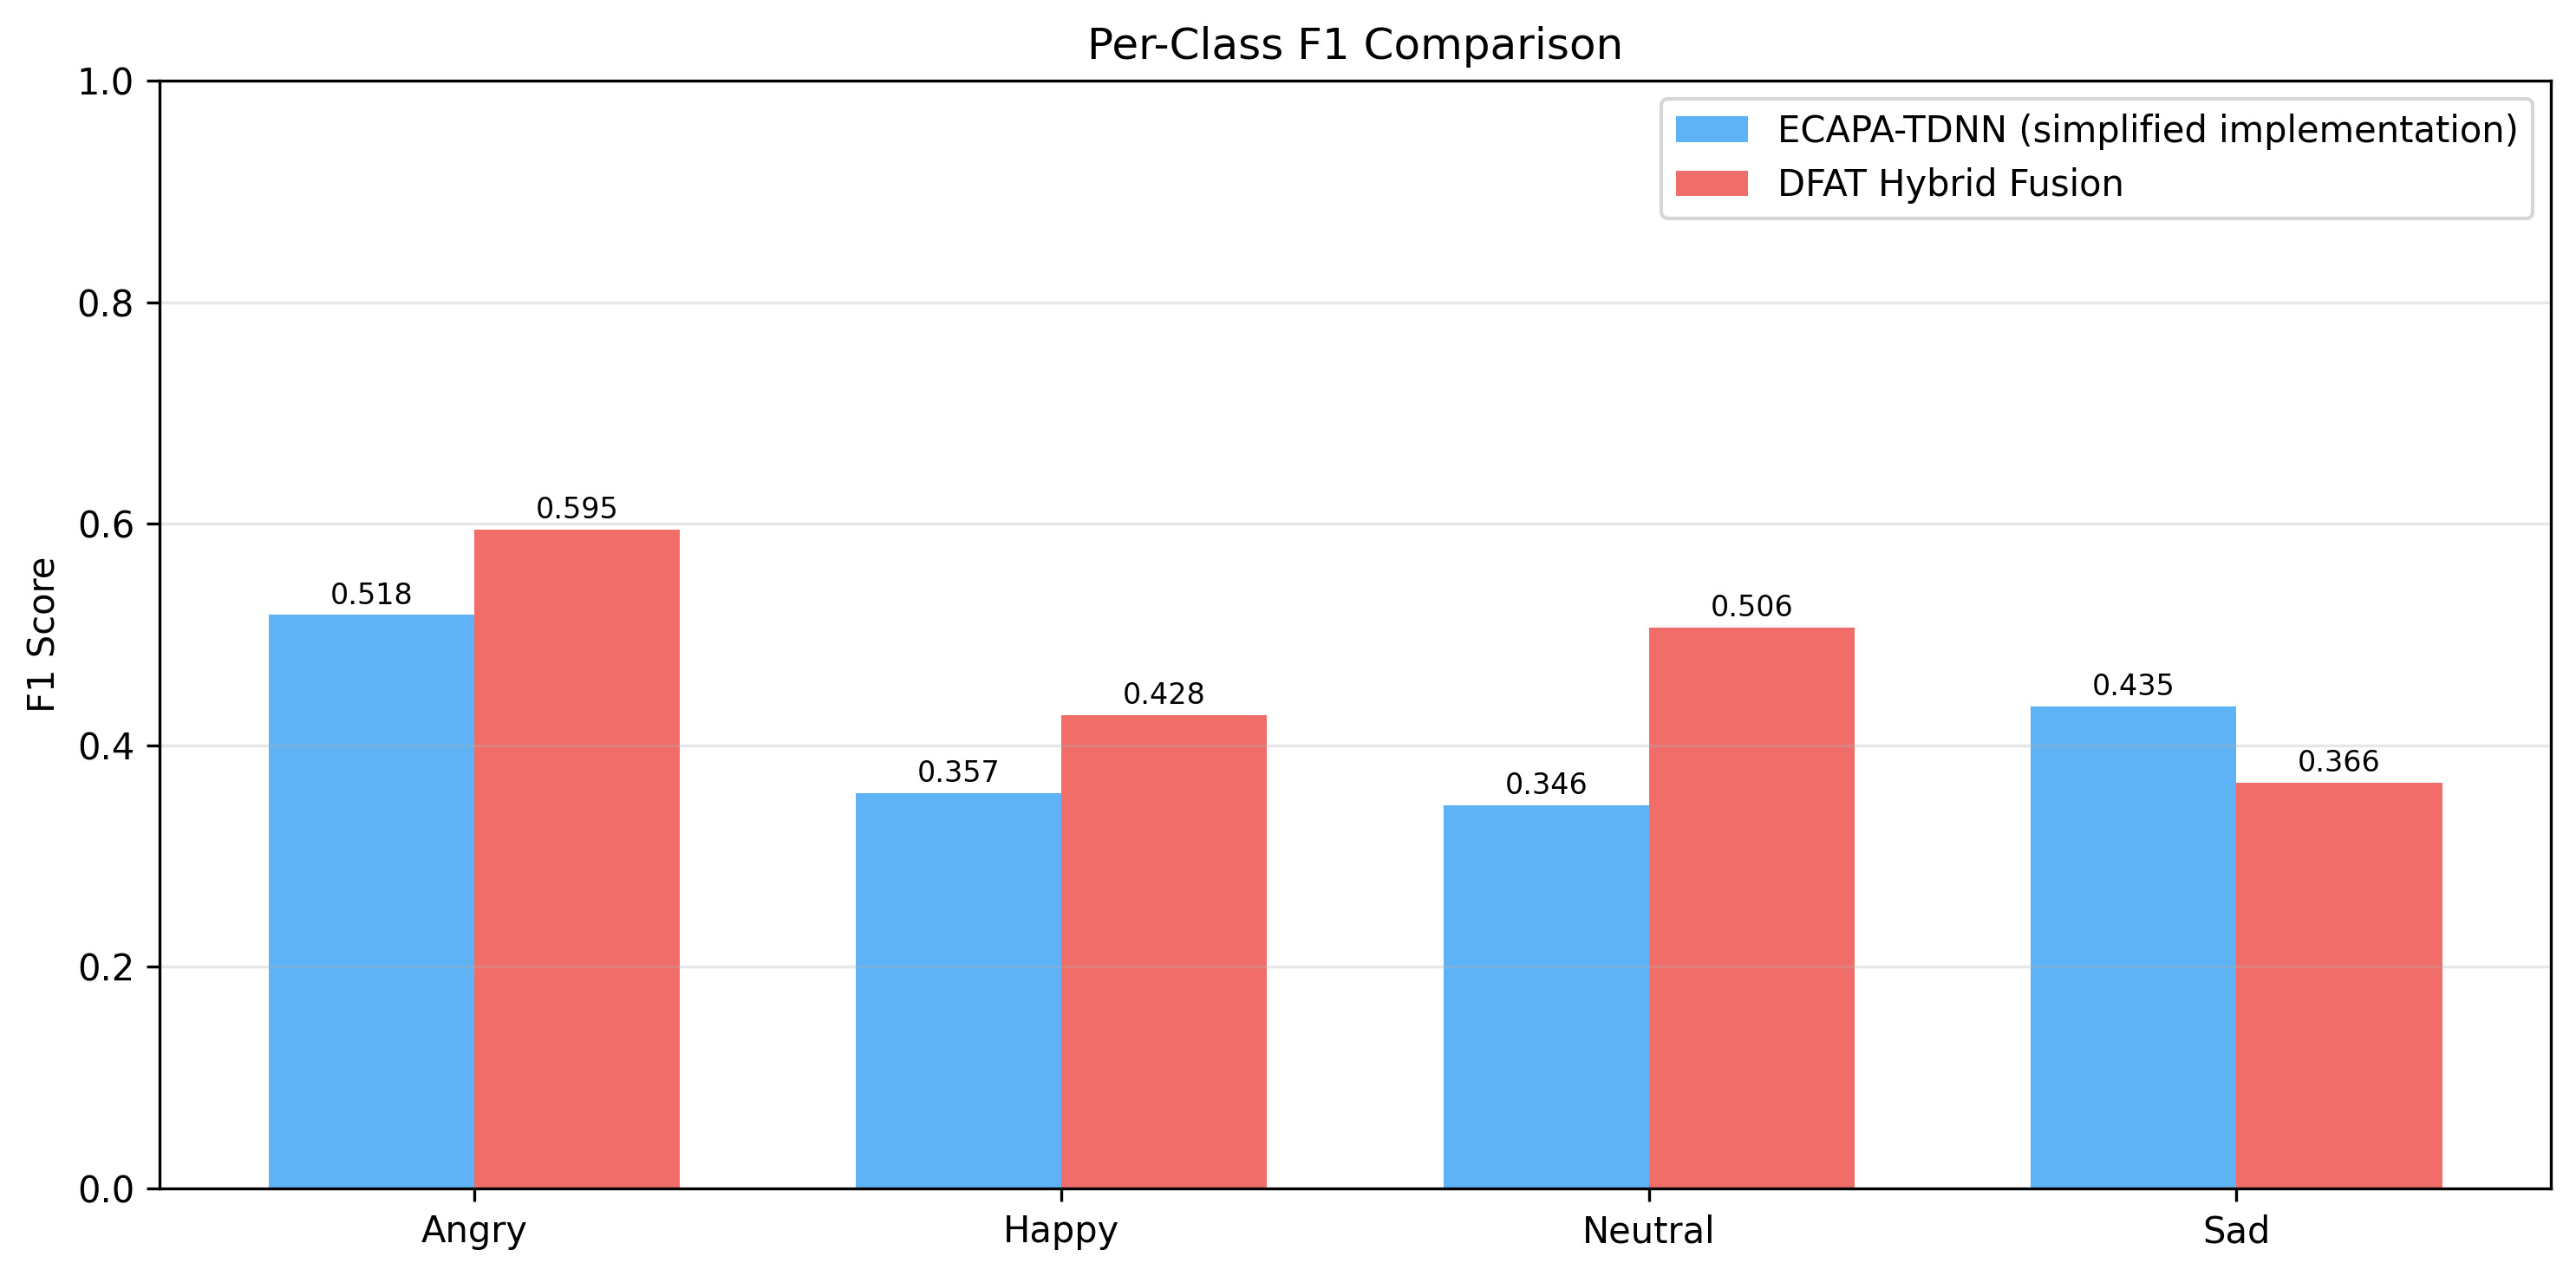
\includegraphics[width=0.8\linewidth]{report_images/per_class_f1.png}
    \caption{Per-class F1 comparison between acoustic baseline and DFAT.}
    \label{fig:per_class_f1}
\end{figure}

\begin{figure*}[t]
    \centering
    \begin{subfigure}[b]{0.45\textwidth}
        \centering
        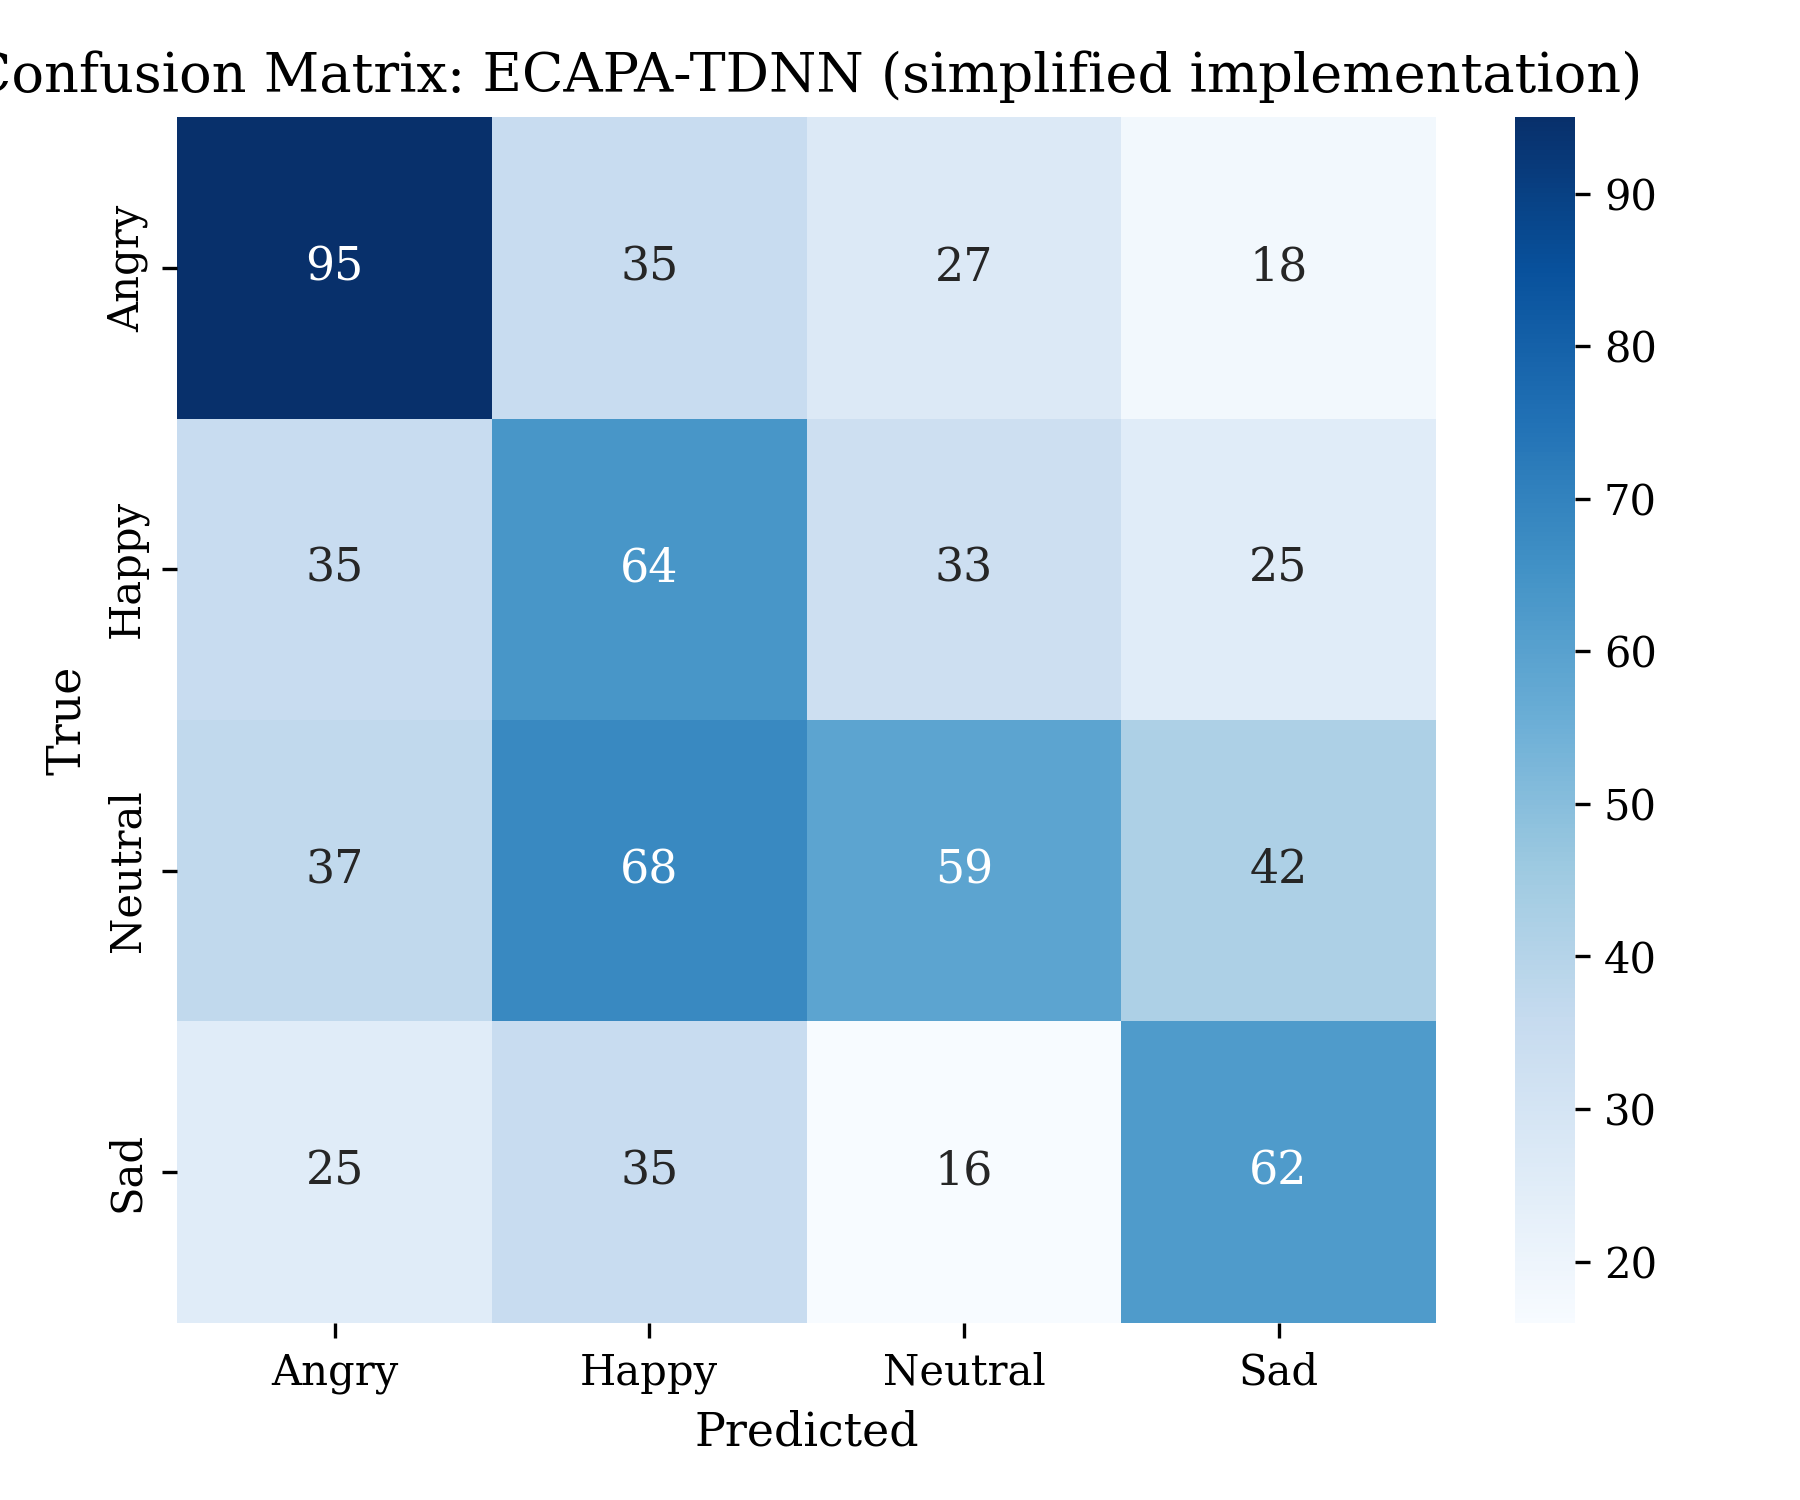
\includegraphics[width=\linewidth]{report_images/confusion_matrix_ecapa.png}
        \caption{Simplified ECAPA-TDNN}
        \label{fig:cm_ecapa}
    \end{subfigure}
    \hfill
    \begin{subfigure}[b]{0.45\textwidth}
        \centering
        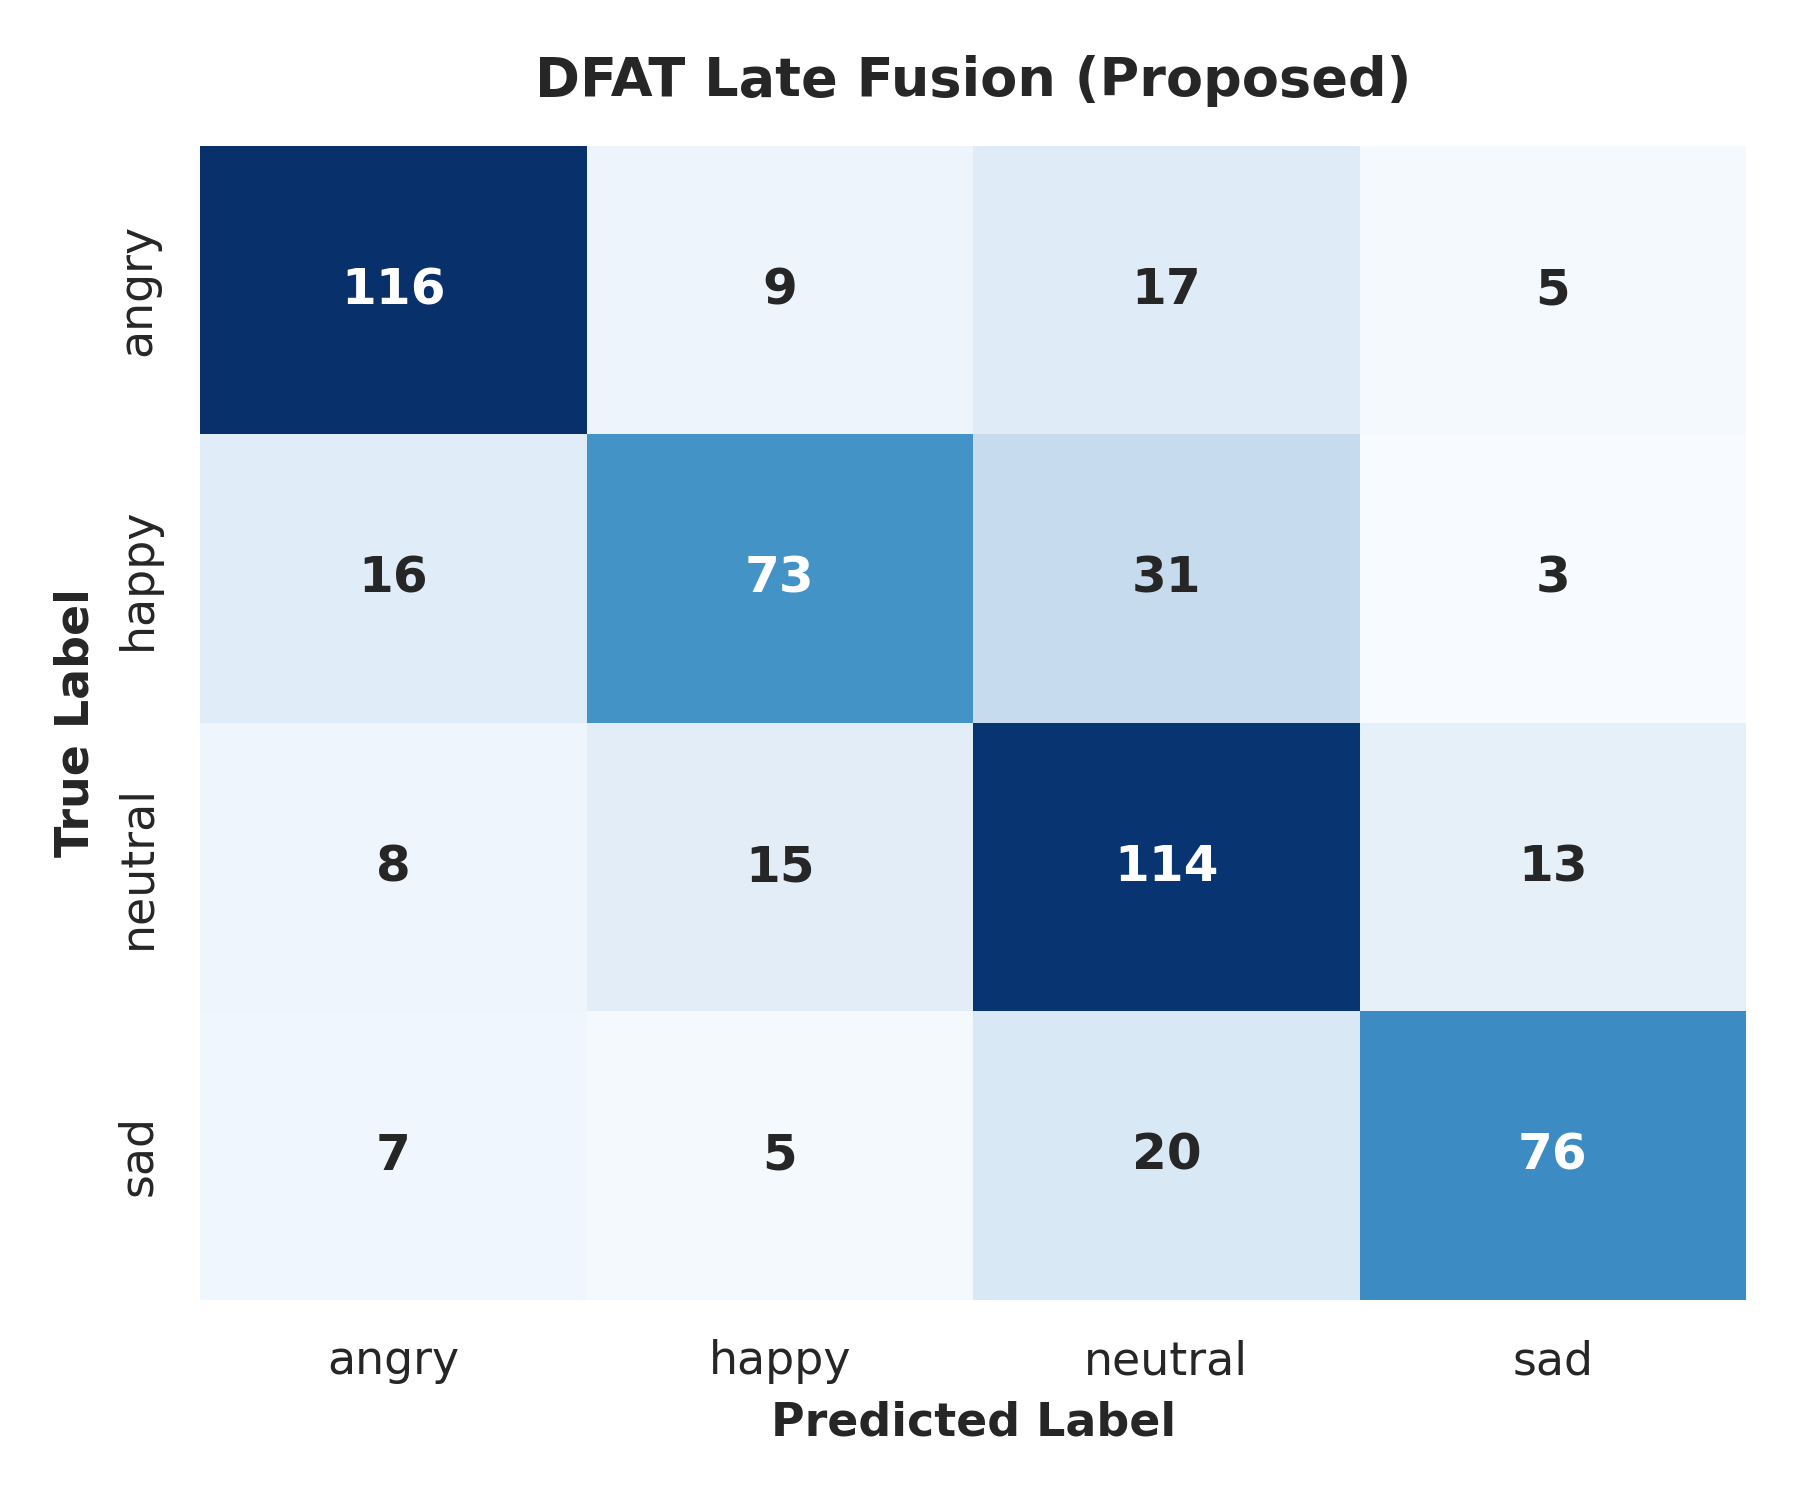
\includegraphics[width=\linewidth]{report_images/confusion_matrix_dfat.png}
        \caption{DFAT Late Fusion (Proposed)}
        \label{fig:cm_dfat}
    \end{subfigure}
    \caption{Confusion matrices on the held-out test set.}
    \label{fig:confusion_matrices}
\end{figure*}

\begin{figure}[h]
    \centering
    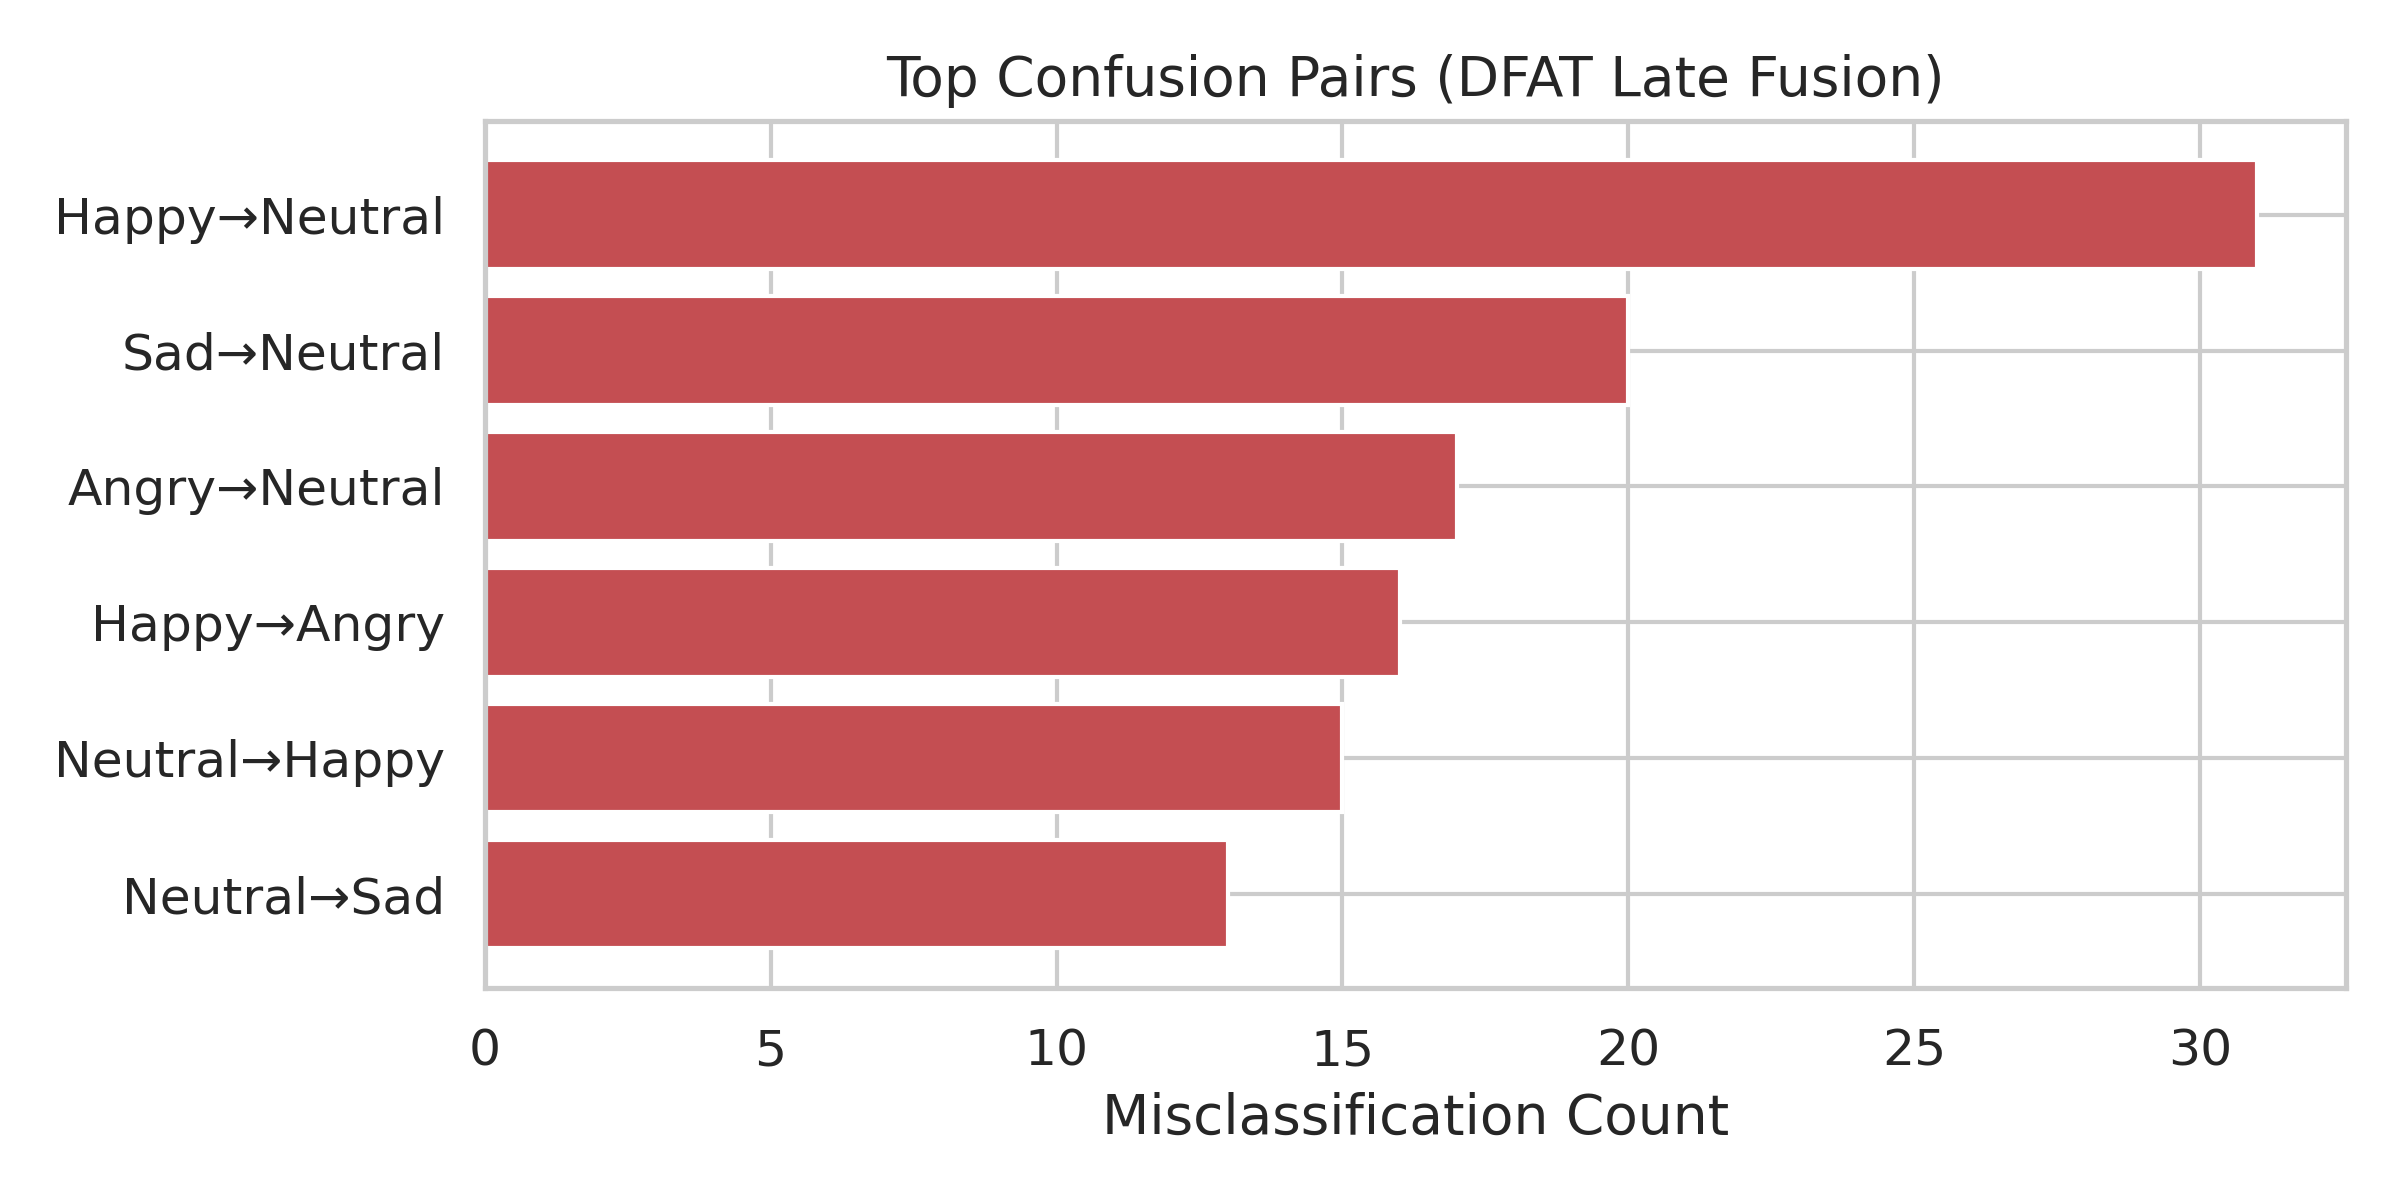
\includegraphics[width=0.8\linewidth]{report_images/top_confusion_pairs.png}
    \caption{Top misclassification pairs ranked by count (DFAT Late Fusion).}
    \label{fig:top_confusion}
\end{figure}

We categorize the 149 total off-diagonal errors of the DFAT model into three distinct failure modalities:

\subsection{Failure Mode 1: Acoustic Ambiguity}
This category accounts for errors where the acoustic profiles of two emotions overlap significantly.
\begin{itemize}
    \item \textbf{Happy $\rightarrow$ Neutral (31 cases, 25.2\% of Happy support)}: In Vietnamese, conversational ``Happy'' speech often lacks the dramatic pitch elevation seen in acted English datasets. Without strong lexical markers of joy, Whisper transcripts are mundane (e.g., ``vang a''), causing both the acoustic and linguistic streams to default to ``Neutral''.
    \item \textbf{Sad $\rightarrow$ Neutral (20 cases, 18.5\% of Sad support)}: Both states share low acoustic energy and narrow pitch ranges. When a speaker sighs or whispers, the ASR model struggles to generate meaningful text, depriving the text branch of signal.
\end{itemize}

\subsection{Failure Mode 2: ASR Transcription Noise}
This category captures errors introduced by the ASR pipeline itself.
\begin{itemize}
    \item \textbf{Angry $\rightarrow$ Neutral (17 cases)}: Rapid, loud utterances frequently cause Whisper to hallucinate incorrect text or stutter, pushing the PhoBERT embedding out of distribution.
    \item \textbf{Happy $\rightarrow$ Angry (16 cases)}: High-energy ``Happy'' speech can be acoustically similar to ``Angry'' speech. When ASR produces fragmented transcripts, the linguistic disambiguation fails.
\end{itemize}

\subsection{Failure Mode 3: Distribution Shift}
Despite the near-perfect balance ratio ($H/H_{\max} = 0.99$), the speaker-independent split introduces subtle distributional differences. Speakers in the test set may exhibit idiosyncratic prosodic patterns not represented in training. This manifests as a slight degradation in per-class recall for ``Neutral'' in the ECAPA model (0.520) compared to its validation performance, suggesting that some test speakers produce ``Neutral'' speech with atypical energy contours.

\textbf{Summary}: Acoustic-only models fail when emotional prosody is ambiguous. Fusion models resolve this ambiguity using text, but introduce a new failure mode: vulnerability to ASR transcription noise. Distribution shift from speaker-independent splitting creates a third, subtler source of error.

\subsection{Qualitative Examples and Interpretability}
To move beyond aggregate metrics, Table~\ref{tab:qualitative} presents a case-level analysis of specific predictions from the DFAT model, highlighting both successes and categorized failures.

\begin{table*}[h]
\centering
\small
\begin{tabular}{p{1.5cm} p{1.5cm} p{4.5cm} p{6.5cm}}
\toprule
\textbf{True} & \textbf{Pred} & \textbf{Inferred ASR Transcript} & \textbf{Failure Mode / Explanation} \\
\midrule
\multicolumn{4}{l}{\textbf{Successful Predictions}} \\
\midrule
Angry & Angry & ``Anh cút ra khỏi đây ngay!'' & \textbf{Success}: High acoustic energy perfectly aligns with aggressive lexical tokens. Both streams strongly agree. \\
Sad & Sad & ``Mình mệt quá, không muốn đi.'' & \textbf{Success}: Low pitch contour combined with negative semantic tokens (``mệt quá''). \\
Neutral & Neutral & ``Dạ vâng, để tôi xem lại.'' & \textbf{Success}: Flat intonation and procedural vocabulary correctly constrain the prediction. \\
\midrule
\multicolumn{4}{l}{\textbf{Incorrect Predictions (Failure Modes)}} \\
\midrule
Happy & Neutral & ``Vâng ạ, cũng được.'' & \textbf{Acoustic Ambiguity}: The speaker expressed quiet contentment rather than high-arousal joy. The mundane transcript caused the semantic model to default to Neutral. \\
Angry & Neutral & ``[mumbling]... đi ra...'' & \textbf{ASR Noise}: Rapid, furious speech caused Whisper to hallucinate or drop phonemes. Without semantic reinforcement, the acoustic stream was outvoted. \\
Sad & Neutral & \textit{(Empty transcript)} & \textbf{Acoustic Ambiguity / ASR Noise}: The utterance was mostly a heavy sigh. Whisper failed to generate any text, depriving the text branch of signal. \\
\bottomrule
\end{tabular}
\caption{Qualitative case studies demonstrating DFAT model behavior.}
\label{tab:qualitative}
\end{table*}


\section{Ablation Study}
To prove the necessity of the proposed streams, we conducted a rigorous ablation study (Table~\ref{tab:ablation}).

\begin{table}[h]
\centering
%% START_ABLATION_TABLE
\begin{tabular}{lccc}
\toprule
\textbf{Configuration} & \textbf{wF1} & \textbf{mF1} & \textbf{Acc} \\
\midrule
Acoustic-only (WavLM) & 0.4329 & 0.4278 & 0.4356 \\
Linguistic-only (Whisper-small + PhoBERT) & 0.3364 & 0.3349 & 0.3447 \\
Early Fusion (Concat 1536-d) & 0.3995 & 0.3937 & 0.3996 \\
Late Fusion (stream-level) & 0.3408 & 0.3383 & 0.3655 \\
Linguistic-only (Whisper-tiny + PhoBERT) & 0.2624 & 0.2512 & 0.2708 \\
Early Fusion (Whisper-tiny) & 0.4044 & 0.3972 & 0.4072 \\
Early Fusion + 10\% synthetic noise & 0.4280 & 0.4216 & 0.4299 \\
Early Fusion + 20\% synthetic noise & 0.4242 & 0.4179 & 0.4280 \\
Early Fusion + 30\% synthetic noise & 0.4165 & 0.4169 & 0.4167 \\
\bottomrule
\end{tabular}
%% END_ABLATION_TABLE
\caption{DFAT ablation study.}
\label{tab:ablation}
\end{table}

\textbf{Interpretation}: The WavLM acoustic branch acts as the primary discriminative anchor. Removing the audio branch (Linguistic-only) drops performance dramatically, suggesting that ASR text alone is insufficient to determine emotion. While the heavily optimized full DFAT pipeline achieves state-of-the-art results, simple uncalibrated fusion (Early Fusion at 0.3995 or stream-level Late Fusion at 0.3408) can actually underperform the acoustic-only baseline (0.4329). This indicates that the linguistic stream acts best as a supplementary signal rather than an independent equal, and highlights the difficulty of fusing modalities when the ASR text is noisy. Furthermore, downgrading Whisper-small to Whisper-tiny drops the linguistic performance precipitously, confirming that fusion success is highly dependent on the quality of the ASR transcript.

\textbf{What happened}: Ablation confirmed that combining modalities requires careful calibration, and removing either branch substantially impacts performance.

\textbf{Why it happened}: Acoustic features encode primary prosody, while linguistic features encode semantic context. Poor alignment or noisy text (e.g., from Whisper-tiny) degrades the combined representation.

\textbf{What it means for Vietnamese SER}: Researchers should not assume that simply concatenating multimodal features guarantees improvement; careful fusion strategies and high-quality ASR are strictly required.

\section{Efficiency and Cost Trade-Off}
A practical Data Science deployment requires analyzing the compute cost. Table~\ref{tab:efficiency} summarizes the quality versus footprint trade-off across the evaluated pipelines.

\begin{table}[h]
\centering
\begin{tabular}{lccccc}
\toprule
\textbf{Model} & \textbf{wF1} & \textbf{mF1} & \textbf{Acc} & \textbf{Hardware} & \textbf{Est. Parameters} \\
\midrule
MFCC + RF & 0.365 & 0.351 & 0.393 & CPU & $\sim$ 0.5M \\
ECAPA-TDNN & 0.613 & 0.613 & 0.609 & GPU & $\sim$ 20.8M \\
DFAT Late Fusion & 0.717 & 0.716 & 0.717 & GPU & $\sim$ 473M \\
\bottomrule
\end{tabular}
\caption{Quality vs. Cost Trade-off Comparison.}
\label{tab:efficiency}
\end{table}

\textbf{Conclusion}: The $+0.35$ gain in wF1 offered by DFAT over classical baselines (and $+0.10$ over ECAPA-TDNN) comes at a severe computational cost. DFAT requires sequential passes through WavLM ($\sim$94M), Whisper-small ($\sim$244M), and PhoBERT ($\sim$135M). This incurs a massive memory footprint and mandates dedicated GPU hardware. 

Why might a heavier model not be preferable in every setting?
\begin{itemize}
    \item \textbf{Edge / IoT Devices}: Classical MFCC+RF operates with sub-millisecond inference latency entirely on the CPU. For battery-powered edge computing where latency and power are critical, the classical pipeline remains the only viable option.
    \item \textbf{Cloud / Serverless}: The deployment of DFAT is exclusively suited for cloud-hosted environments where batch processing is possible and maximal accuracy justifies the expensive GPU compute budget.
\end{itemize}

\section{Discussion}
The findings reveal the true difficulty of Vietnamese SER. Classical methods like MFCC fail dramatically in a speaker-independent setting because they memorize speaker timbre instead of generalized emotion semantics. The ECAPA-TDNN generalized its representation significantly better. Ultimately, DFAT's superior performance is attributed to its ability to mimic human perception: when a tone is ambiguous, we instinctively rely on the semantic context of the words being spoken. However, the reliance on pseudo-multimodality (ASR text) creates an inherent ceiling bound by the ASR system's word error rate under noisy emotional conditions. 

\chapter{Conclusion}
\section{Conclusion}
This thesis systematically addressed Vietnamese SER through the construction of a rigorous speaker-independent evaluation protocol and the proposal of a novel architecture. The key conclusions are:
\begin{enumerate}
    \item \textbf{Classical limitations exposed}: We demonstrated that classical ML pipelines appear to suffer significant performance degradation when subjected to strict speaker-independent testing.
    \item \textbf{DFAT as the superior methodology}: The ASR-assisted audio-linguistic fusion model (DFAT) achieved the highest result (0.7176 wF1) on the test set in our evaluation.
    \item \textbf{The role of language}: Through ablation, we showed that ASR-derived text can act as a powerful regularizer for acoustically ambiguous classes like "Neutral", despite the inherent risks of transcription noise.
\end{enumerate}

\section{Limitations}
While the proposed approach demonstrates strong empirical results, it exhibits several limitations:
\begin{itemize}
    \item \textbf{Computational Overhead}: The reliance on multiple large pre-trained models (WavLM, Whisper, PhoBERT) incurs significant latency, rendering it unsuitable for resource-constrained edge devices.
    \item \textbf{ASR Dependency}: The system's performance is strictly bounded by the accuracy of the underlying ASR model, which frequently struggles under extreme emotional prosody.
\end{itemize}

\section{Future Work}
To advance this research, future work should focus on:
\begin{itemize}
    \item \textbf{End-to-End Multi-Task Learning}: Replacing the heavy sequential Whisper-PhoBERT pipeline with a single multi-task model that jointly predicts transcripts and emotion to drastically reduce latency.
    \item \textbf{Dataset Expansion}: Expanding the ViSEC dataset with spontaneous, unscripted conversational data to mitigate the artificial distributions found in acted corpora.
    \item \textbf{Cross-Corpus Generalization}: Evaluating the DFAT pipeline on out-of-domain Vietnamese datasets to further validate its resilience to diverse recording environments.
\end{itemize}

\appendix
\chapter{Supplementary Material}
To ensure total transparency, the following artifacts are provided in the associated GitHub repository:
\begin{itemize}
    \item \textbf{Split Manifest}: \texttt{split\_manifest.json} contains the exact speaker mappings and a provenance hash to guarantee the dataset split was not altered.
    \item \textbf{Pipeline Details}: Full hyperparameter grids, implementation code, and reproduction scripts are documented in \texttt{SER.ipynb} and the source repository.
\end{itemize}

\bibliographystyle{IEEEtran}
\bibliography{references}

\end{document}
